\begin{frame}{[\textbf{Chapter 3}] 結合位相振動子系}
  \begin{block}{大域結合位相振動子モデル}
  \centering
  $\displaystyle\frac{\diff\theta_{i}}{\diff t}=\omega_{i}+\frac{K}{N}\sum_{j=1}^{N}\Gamma(\theta_{j}-\theta_{i})$
  \begin{itemize}
    \item $\omega_{i}\sim g(\omega)$: \textbf{自然振動数分布$g(\omega)$からサンプル}
    \item $K$: 結合定数
    \item $\Gamma(\theta)$: 結合関数(周期$2\pi$)
  \end{itemize}
  \end{block}
  %どれほど同期しているかを表すパラメータ
  \checkmark \textbf{秩序変数}: 同期の強さを表すパラメータ
  \begin{align*}
    r=\left|\frac{1}{N}\sum_{j=1}^{N}e^{i\theta_{j}}\right|
  \end{align*}
  \begin{figure}
    \centering
    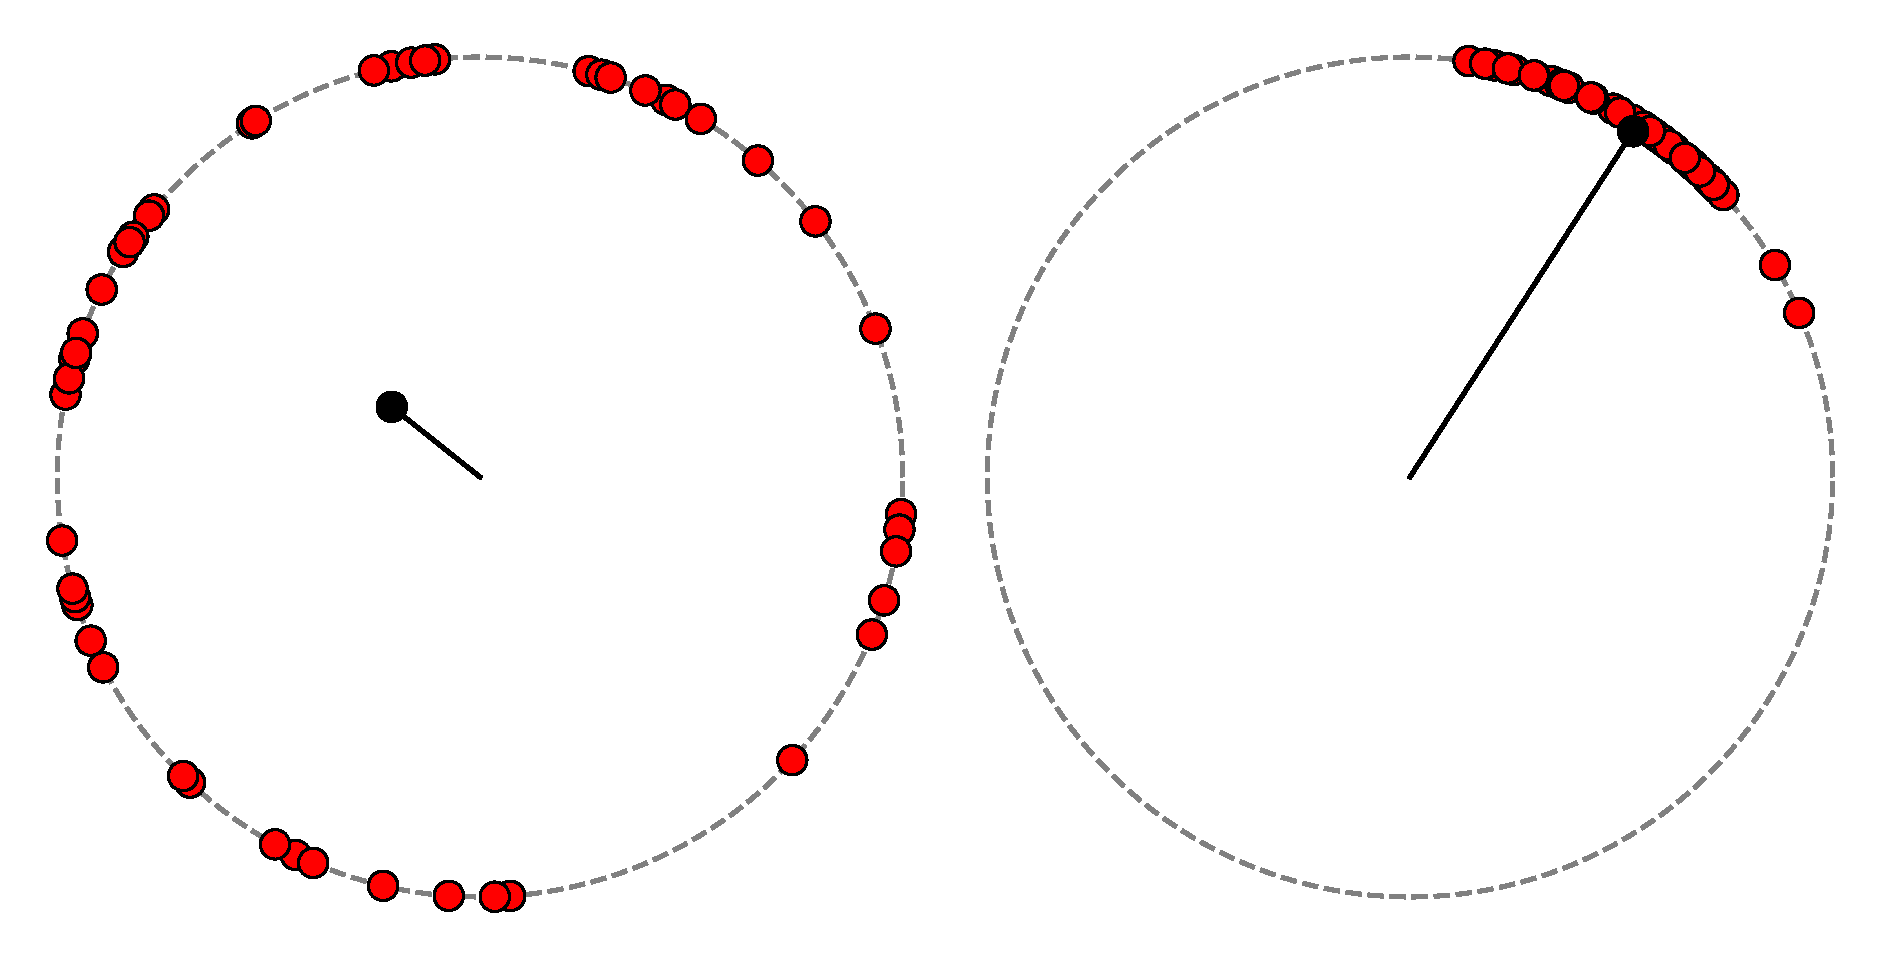
\includegraphics[width=0.4\textwidth]{figs/sync_notsync.pdf}
  \end{figure}
\end{frame}

\begin{frame}\frametitle{分岐図と臨界指数}
%  \begin{block}{臨界指数}
%  \begin{itemize}
%  \item もともと統計力学で研究されてきたもの
%  \item モデルの詳細には依存せず、普遍的な性質のみに依存すると考えられている。
%  \begin{itemize}
%    \item システムの次元
%    \item 相互作用の範囲
%  \end{itemize}
%  \end{itemize}
%  \end{block}
%  \begin{itemize}
%    \item 臨界点$\Kc$周りの立ち上がり
%    \begin{align*}
%      r\sim(K-\Kc)^{\beta}
%    \end{align*}
%    \item $\beta$: 臨界指数
%%    \item 臨界現象の背景には何らかの非自明な数理的構造があるとされている。
%%    \begin{itemize}
%%      \item 2次元Isingモデルの臨界現象の背景には\textbf{共形場理論}と呼ばれる数理的な構造がある。
%%      \item \textbf{Loewner微分方程式}とも関係があるらしい。
%%    \end{itemize}
%    \item $g(\omega)=\dfrac{\Delta}{\pi(\omega^{2}+\Delta^{2})}$(\textbf{Lorentz分布})のとき$\Kc=2\Delta$として
%    \begin{align*}
%      r=\sqrt{1-\frac{\Kc}{K}}\quad\Rightarrow\quad\beta=\frac{1}{2}
%    \end{align*}
%    \item 他の$g(\omega)$のときは??
%    \item 他の結合関数のときは??
%  \end{itemize}
  \begin{figure}
    \centering
    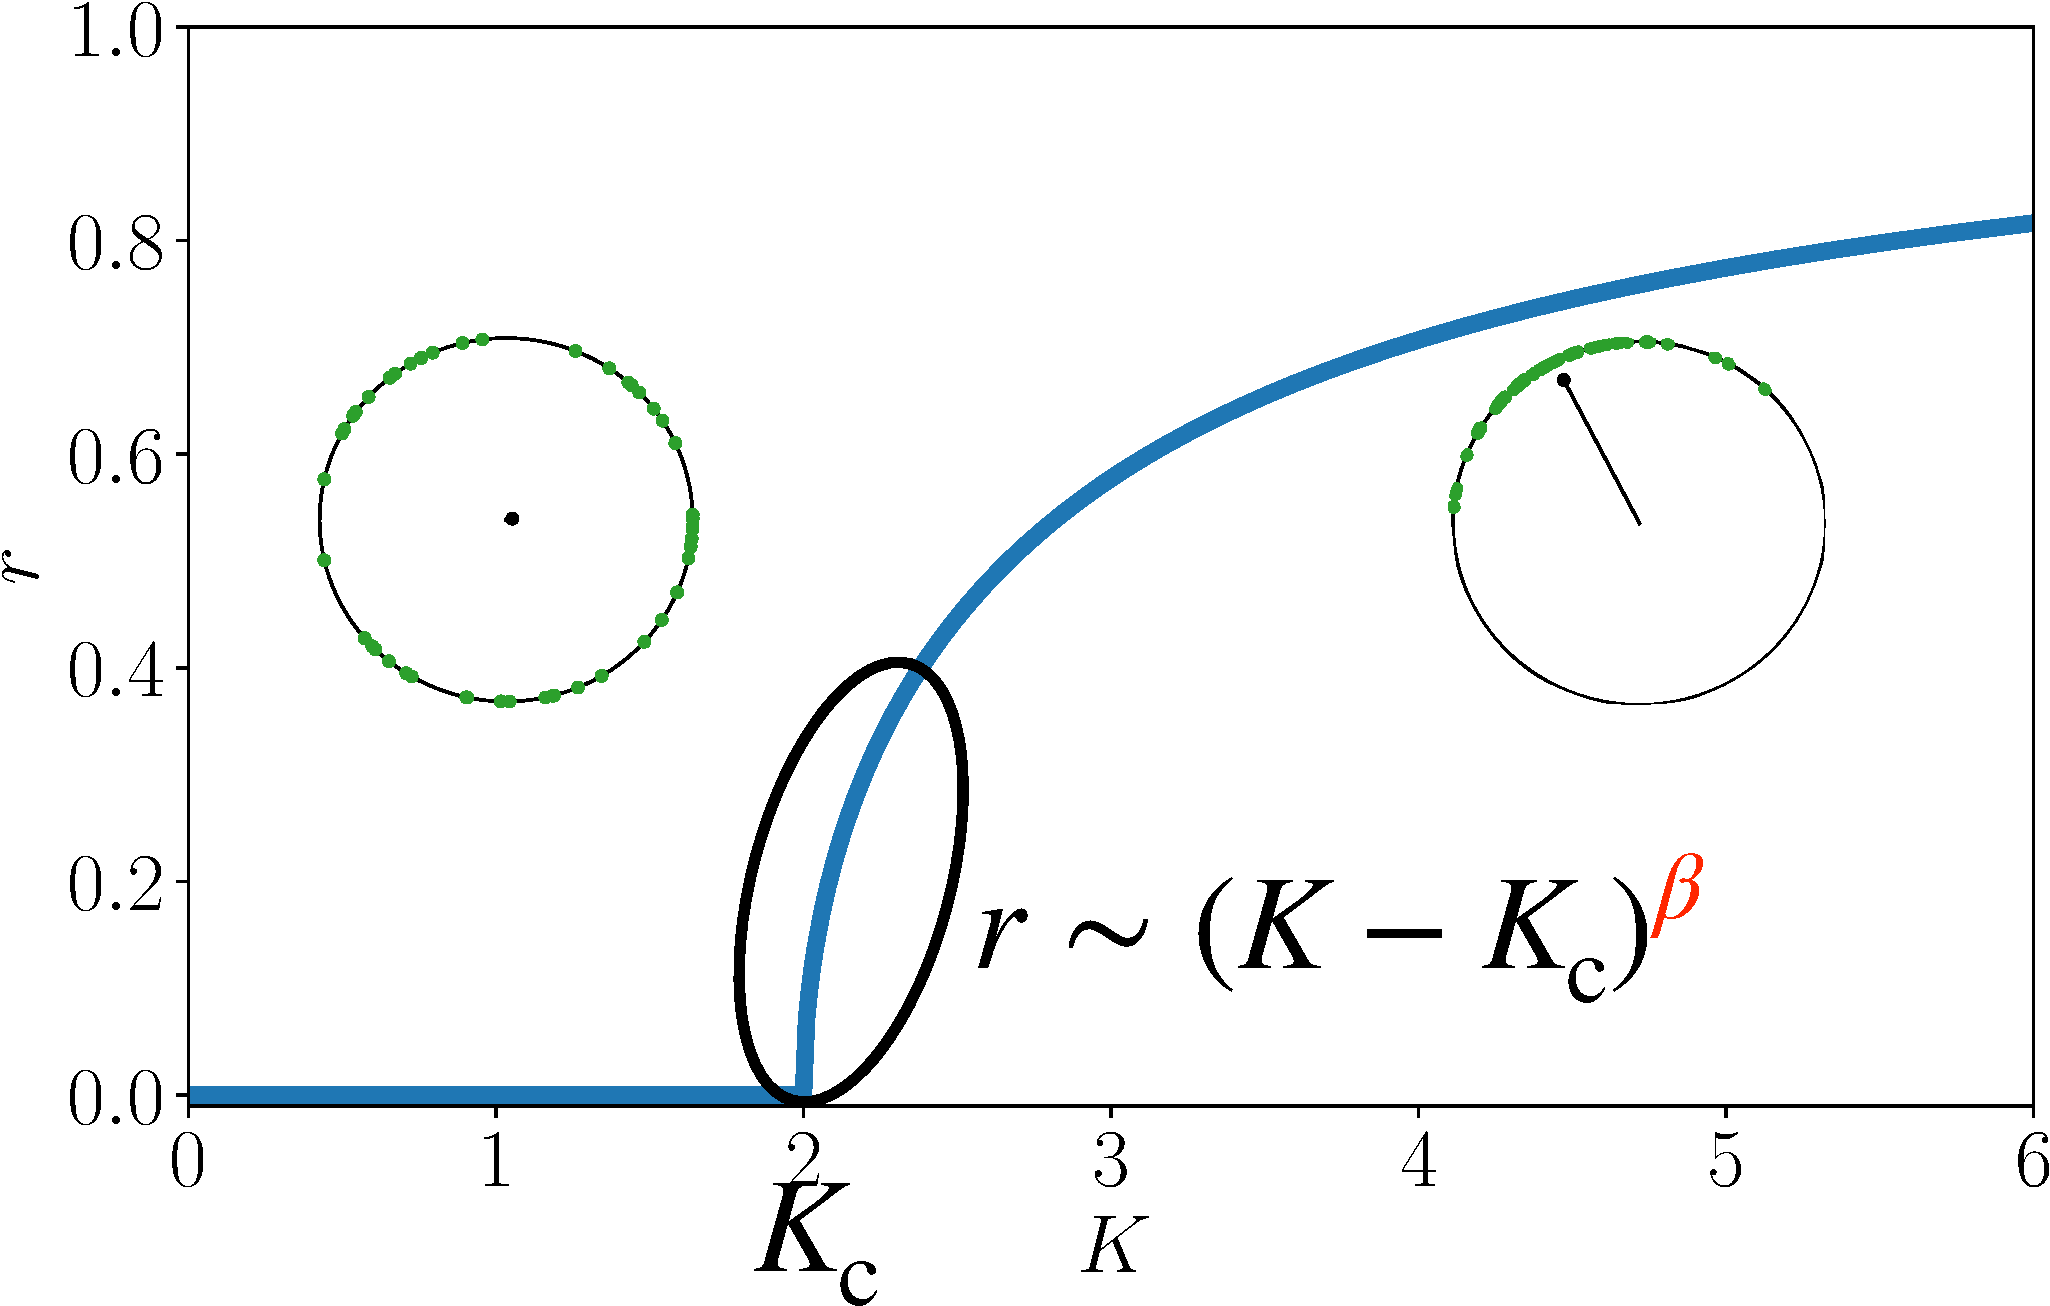
\includegraphics[scale=0.3]{figs/bif_exp-crop.pdf}
  \end{figure}
  \begin{itemize}
    \item $N\to\infty$での連続転移の臨界点近傍での立ち上がり: 臨界指数$\color{red}\beta$
    \begin{itemize}
      %\item 臨界指数は統計力学でよく研究され、\textbf{普遍性(universality)}を記述する
      \item 臨界指数は統計力学でよく研究されている
      \item 分布関数$g(\omega)$、結合関数$\Gamma(\theta)$による依存性
    \end{itemize}
  \end{itemize}
\end{frame}

%\begin{frame}\frametitle{分布関数$g(\omega)$と結合関数$\Gamma(\theta)$}
%  \begin{itemize}
%    \item 分布関数
%    \begin{align*}
%      g_{\color{red}n}(\omega)=\dfrac{n\Delta}{\Gamma(1/2n)}e^{-(\Delta\omega)^{2n}}
%    \end{align*}
%    \begin{itemize}
%      \item ${\color{red}n}=1$: ガウス分布
%      \item マクローリン展開: $g_{n}(\omega)=g_{n}(0)-C_{n}\omega^{\color{red}2n}+\cdots$
%    \end{itemize}
%    \begin{figure}
%      \centering
%      \includegraphics[scale=0.4]{gn.pdf}
%    \end{figure}
%    \item 結合関数
%    \begin{align*}
%      \Gamma(\theta)=\sin\theta+{\color{blue}a}\sin2\theta
%    \end{align*}
%    \begin{itemize}
%      \item ${\color{blue}a}=0$: 蔵本モデル
%%      \begin{align*}
%%        \frac{\diff\theta_{i}}{\diff t}=\omega_{i}+\frac{K}{N}\sum_{j=1}^{N}\sin(\theta_{j}-\theta_{i})
%%      \end{align*}
%    \end{itemize}
%  \end{itemize}
%\end{frame}

%\begin{frame}\frametitle{自然振動数分布の族}
%  \begin{align*}
%    &g^{(L)}_{n}(\omega)=\dfrac{n\sin(\pi/2n)}{\pi}\dfrac{\Delta^{2n-1}}{\omega^{2n}+\Delta^{2n}}\\
%    &g^{(G)}_{n}(\omega)=\dfrac{n\Delta}{\Gamma(1/2n)}e^{-(\Delta\omega)^{2n}}
%    \end{align*}
%    \begin{figure}
%    \centering
%    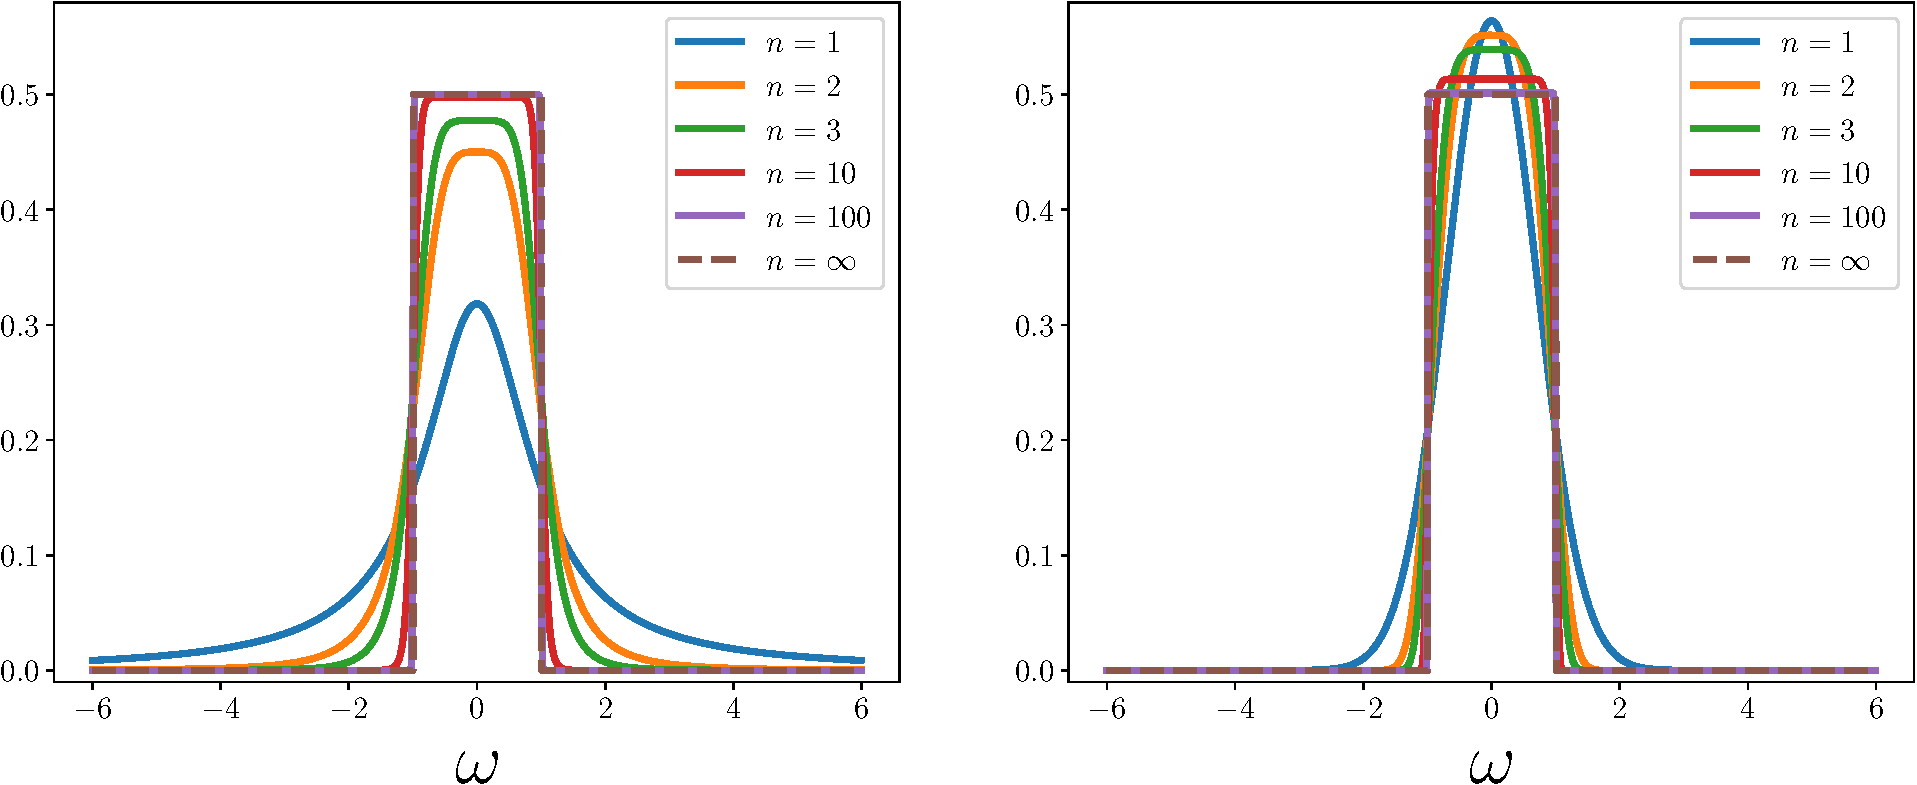
\includegraphics[scale=0.25]{figs/g_omega-crop.pdf}
%    \end{figure}
%    \begin{itemize}
%    \item Lorentz分布とGauss分布の一般化
%    \item $\omega=0$まわりの展開
%    \[
%    g_{n}(\omega)=g_{n}(0)-C_{n}\omega^{\red{2n}}+\cdots
%    \]
%    \item $\beta=\dfrac{1}{2n}$
%    \end{itemize}
%\end{frame}
%
%\begin{frame}\frametitle{$n=\infty$}
%  \begin{align*}
%    r-r_{\mathrm{c}}\propto(K-K_{\mathrm{c}})^{2/3}
%  \end{align*}
%  \begin{figure}
%    \begin{center}
%      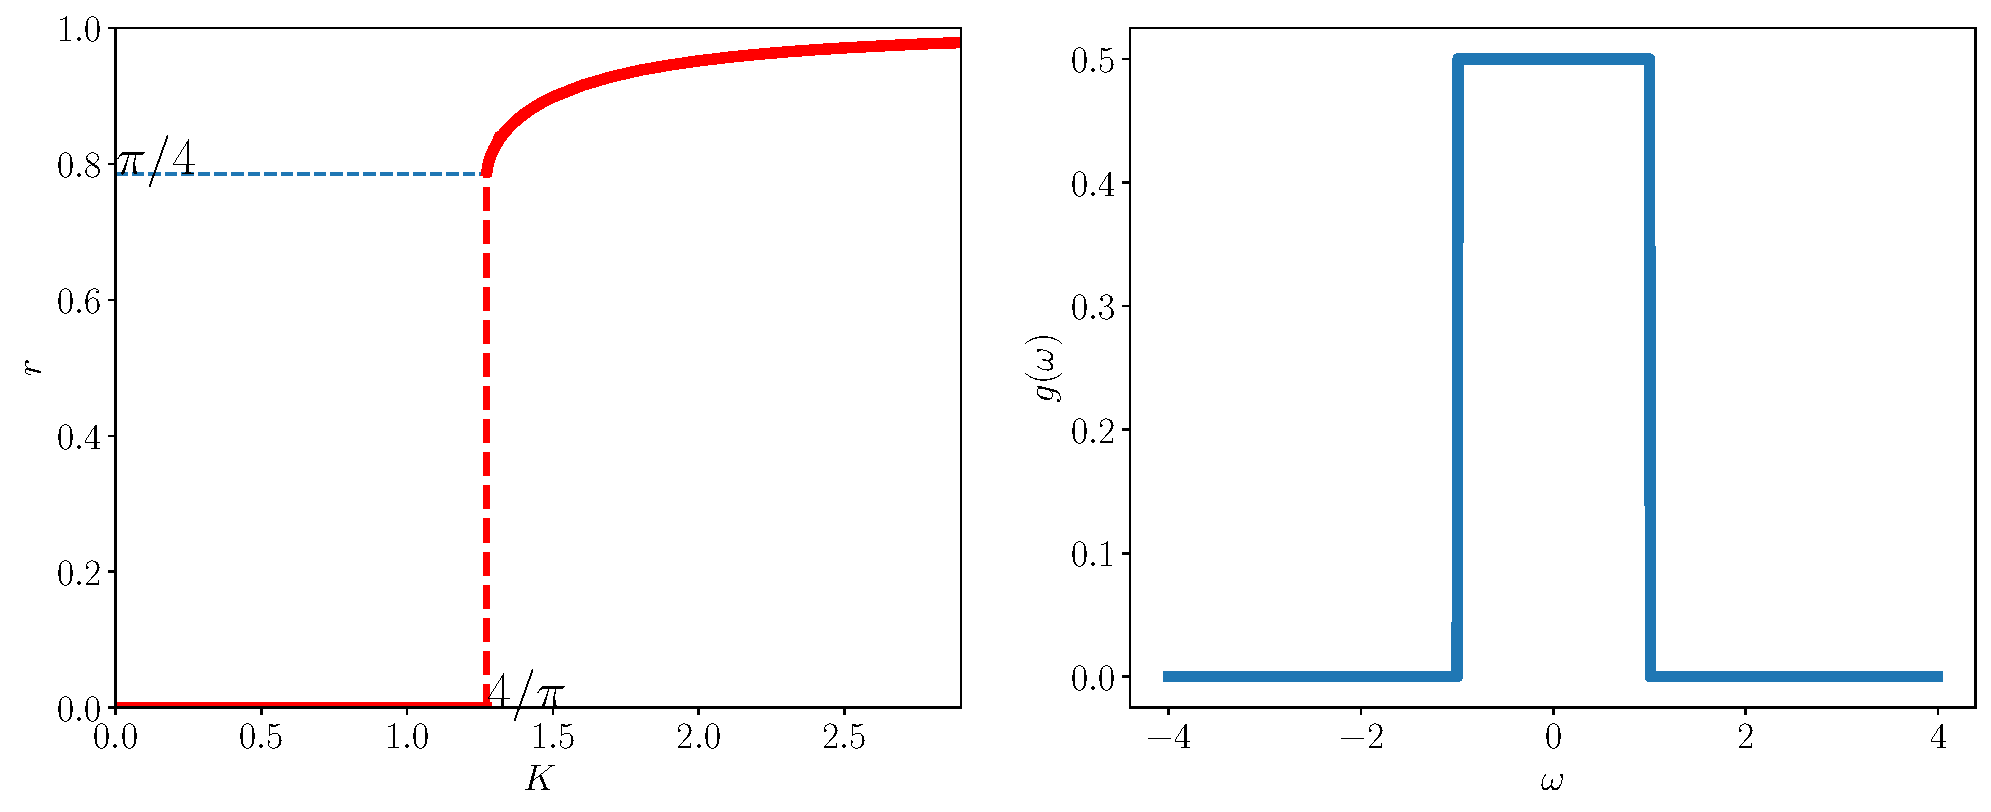
\includegraphics[scale=0.3]{figs/bif-n-inf.pdf}
%    \end{center}
%  \end{figure}
%  \begin{itemize}
%    \item 臨界点でjumpが見られる
%    \item $\beta=\dfrac{2}{3}$
%  \end{itemize}
%\end{frame}
%
%\begin{frame}\frametitle{$\sin2\theta$を付け加える}
%  \begin{align*}
%    \frac{\diff\theta_{i}}{\diff t}=\omega_{i}+\frac{K}{N}\sum_{j=1}^{N}[\sin(\theta_{j}-\theta_{i})+\blue{a\sin2(\theta_{j}-\theta_{i})}]
%    \end{align*}
%    \begin{figure}
%    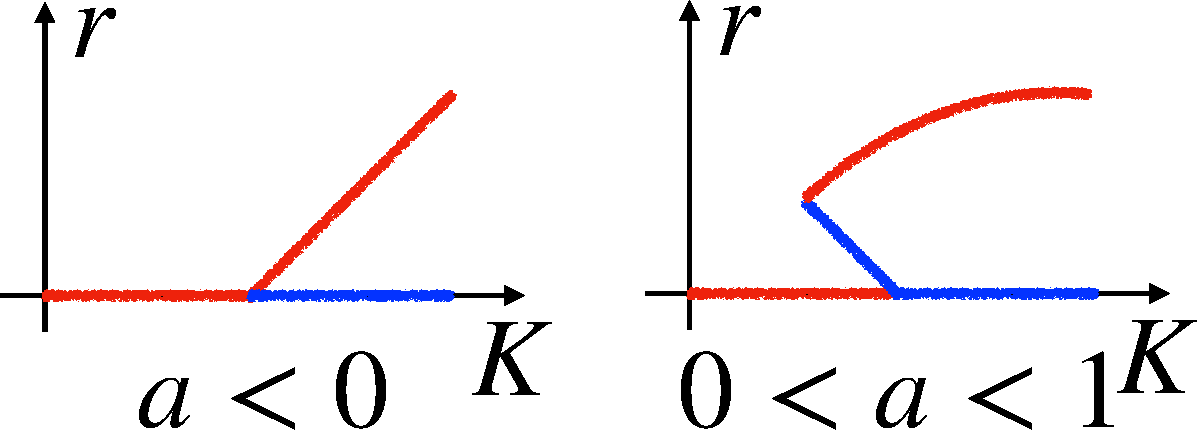
\includegraphics[scale=0.3]{figs/sin2-crop.pdf}
%    \end{figure}
%  \begin{itemize}
%%    \item \textbf{中心多様体縮約}を用いて$\beta=1$であることが示されている[Crawford 1995,Chiba 2011]。
%%    \begin{align*}
%%      &r\sim\frac{2(1-a)}{\Kc^{3}Ca}(K-\Kc)^{\red{1}}+\cdots\\
%%      &C=\mathcal{PV}\int_{\mathbb{R}}\diff\omega\frac{g'(\omega)}{\omega}
%%    \end{align*}
%    \item $a<0$で一山対称の$g(\omega)$のとき
%    \begin{align*}
%      \beta=1
%    \end{align*}
%  \end{itemize}
%\end{frame}

\begin{frame}\frametitle{臨界指数}
%  \begin{wrapfigure}[2]{R}[15pt]{0.5\textwidth}
%    \centering
%    \includegraphics[scale=0.3]{gn.pdf}
%  \end{wrapfigure}
%  \begin{align*}
%    &\Gamma(\theta)=\sin\theta+{\color{blue}a}\sin2\theta\\
%    &g_{n}(\omega)=\dfrac{n\Delta}{\Gamma(1/2n)}e^{-(\Delta\omega)^{2n}}=g_{n}(0)-C_{n}\omega^{\red{2n}}+\cdots
%  \end{align*}
\begin{columns}
  \begin{column}{0.36\linewidth}
    $\Gamma(\theta)=\sin\theta+{\color{blue}a}\sin2\theta$\\
    $g_{\color{red}n}(\omega)=\dfrac{ne^{-(\omega/\Delta)^{\color{red}2n}}}{\Gamma(1/2n)\Delta}$
  \end{column}
  \begin{column}{0.56\linewidth}
    \begin{figure}
      \centering
      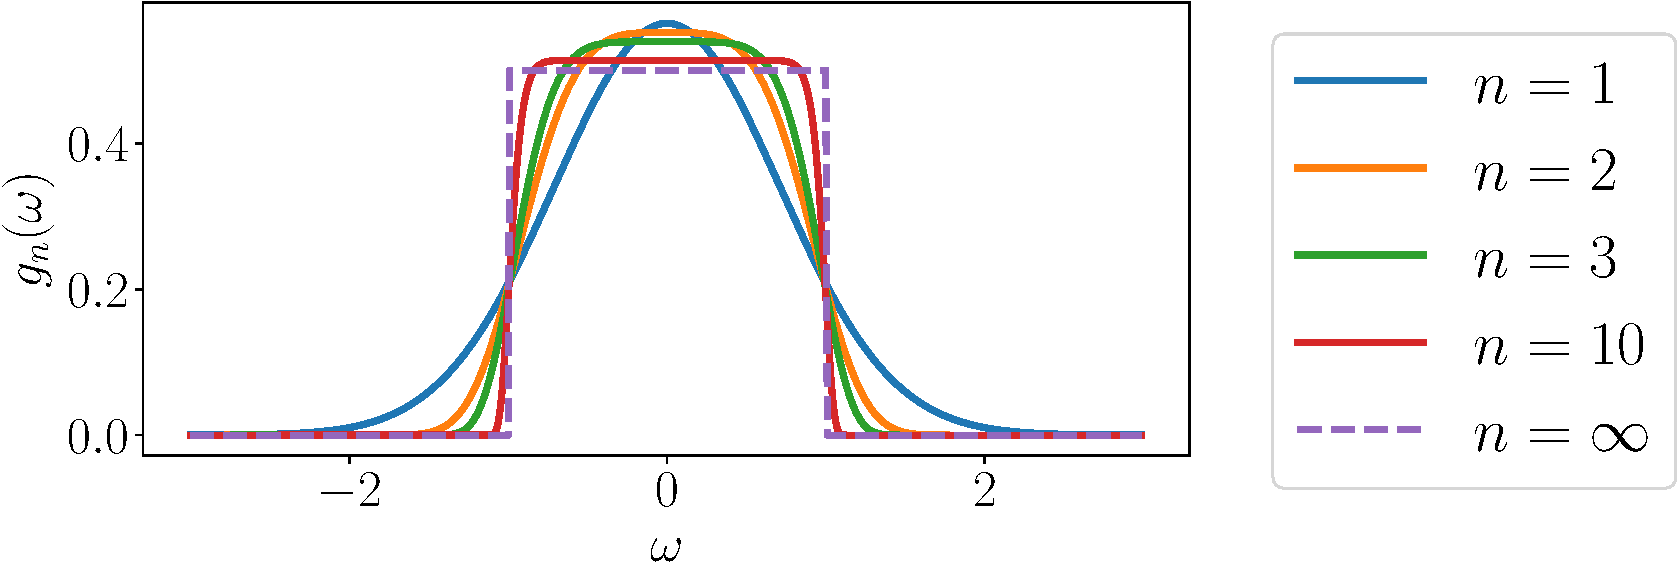
\includegraphics[width=\linewidth]{figs/gn-crop.pdf}
    \end{figure}
  \end{column}
\end{columns}
  %$g_{n}(\omega)=\dfrac{n\Delta}{\Gamma(1/2n)}e^{-(\Delta\omega)^{2n}}=g_{n}(0)-C_{n}\omega^{\red{2n}}+\cdots$
  \begin{table}[htbp]
    \begin{center}
      \begin{tabular}{c||c|c|c}\hline\hline
       & \multicolumn{3}{c}{all-to-all} \\\hline
       & $a<0$ & $a=0$ & $a>0$ \\\hline\hline
      $n=1$ & \multirow{3}{*}{\begin{tabular}{c}$1$\\(Chiba 2011)\end{tabular}} & \begin{tabular}{c}$1/2$\\(Kuramoto 1975)\end{tabular} & \multirow{3}{*}{\begin{tabular}{c}(不連続)\\(Chiba 2011)\end{tabular}} \\\cline{3-3}
      $n\geq 2$ & & \begin{tabular}{c}$1/(2n)$\\(Basanarkov 2007)\end{tabular} & \\\cline{3-3}
      $n=\infty$ & &  \begin{tabular}{c}(不連続)\\(Pazo 2005)\end{tabular} &  \\\hline\hline
      \end{tabular}
    \end{center}
  \end{table}
  \begin{itemize}
    \item 理論的な導出はモデルの\textbf{全結合性}に強く依存
    \item 本研究: \underline{\textbf{現実に即したネットワークにおける臨界指数を調べる}}
  \end{itemize}
\end{frame}

%$1$\\[Chiba et al. 2011]}\end{tabular}

%\begin{frame}\frametitle{スモールワールドネットワーク}
%  \begin{itemize}
%    \item 現実のネットワークに関する研究
%    \begin{itemize}
%      \item ``6次の隔たり''
%      \item 強いクラスター化
%    \end{itemize}
%  \end{itemize}
%  \begin{block}{スモールワールド性}
%    \begin{itemize}
%      \item 平均ノード間距離$\langle l\rangle$がノード数$N$に対して$\langle l\rangle\ll N$
%      \item 平均クラスター係数がノード数$N$に依存しない
%    \end{itemize}
%  \end{block}
%  \begin{itemize}
%    \item \textbf{Watts-Strogatz model}: スモールワールド性を記述する代表的なモデル[Watts and Strogatz 1998]
%    \item \red{$O(N)$}本の枝を持つ(全結合グラフは$O(N^{2})$)
%  \end{itemize}
%  \begin{figure}
%    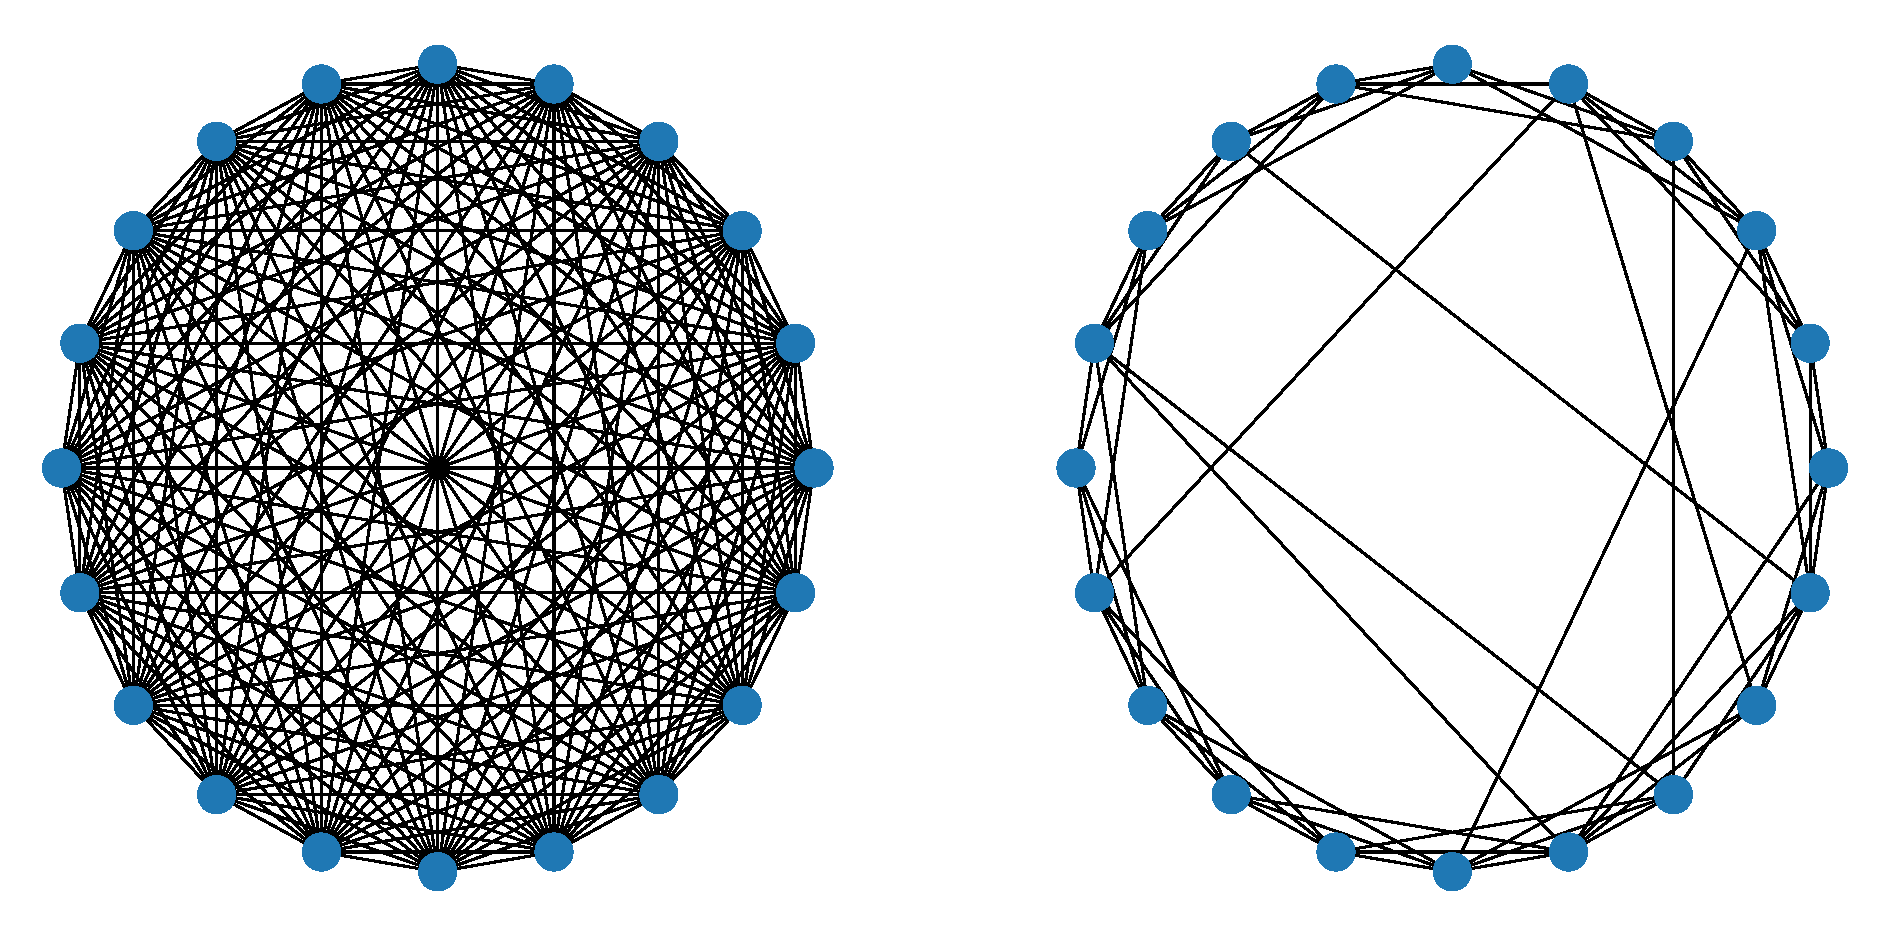
\includegraphics[width=8cm]{figs/mf_sw.pdf}
%  \end{figure}
%\end{frame}

%\begin{frame}\frametitle{Watts--Strogatz model}
%\begin{block}{アルゴリズム}
%  \begin{itemize}
%    \item[1] $N$個の頂点を持つ$k$-隣接グラフを生成する。
%    \item[2] $kN$本の枝のそれぞれに対して、確率$p$でエッジの一方(ランダムに選ぶ)の結合を切り離し、$N$頂点の中からランダムに選ばれた頂点につなぎ替える。
%    ただし、自己ループや多重エッジができないようにする。 
%  \end{itemize}
%\end{block}
%\begin{figure}
%  \begin{center}
%    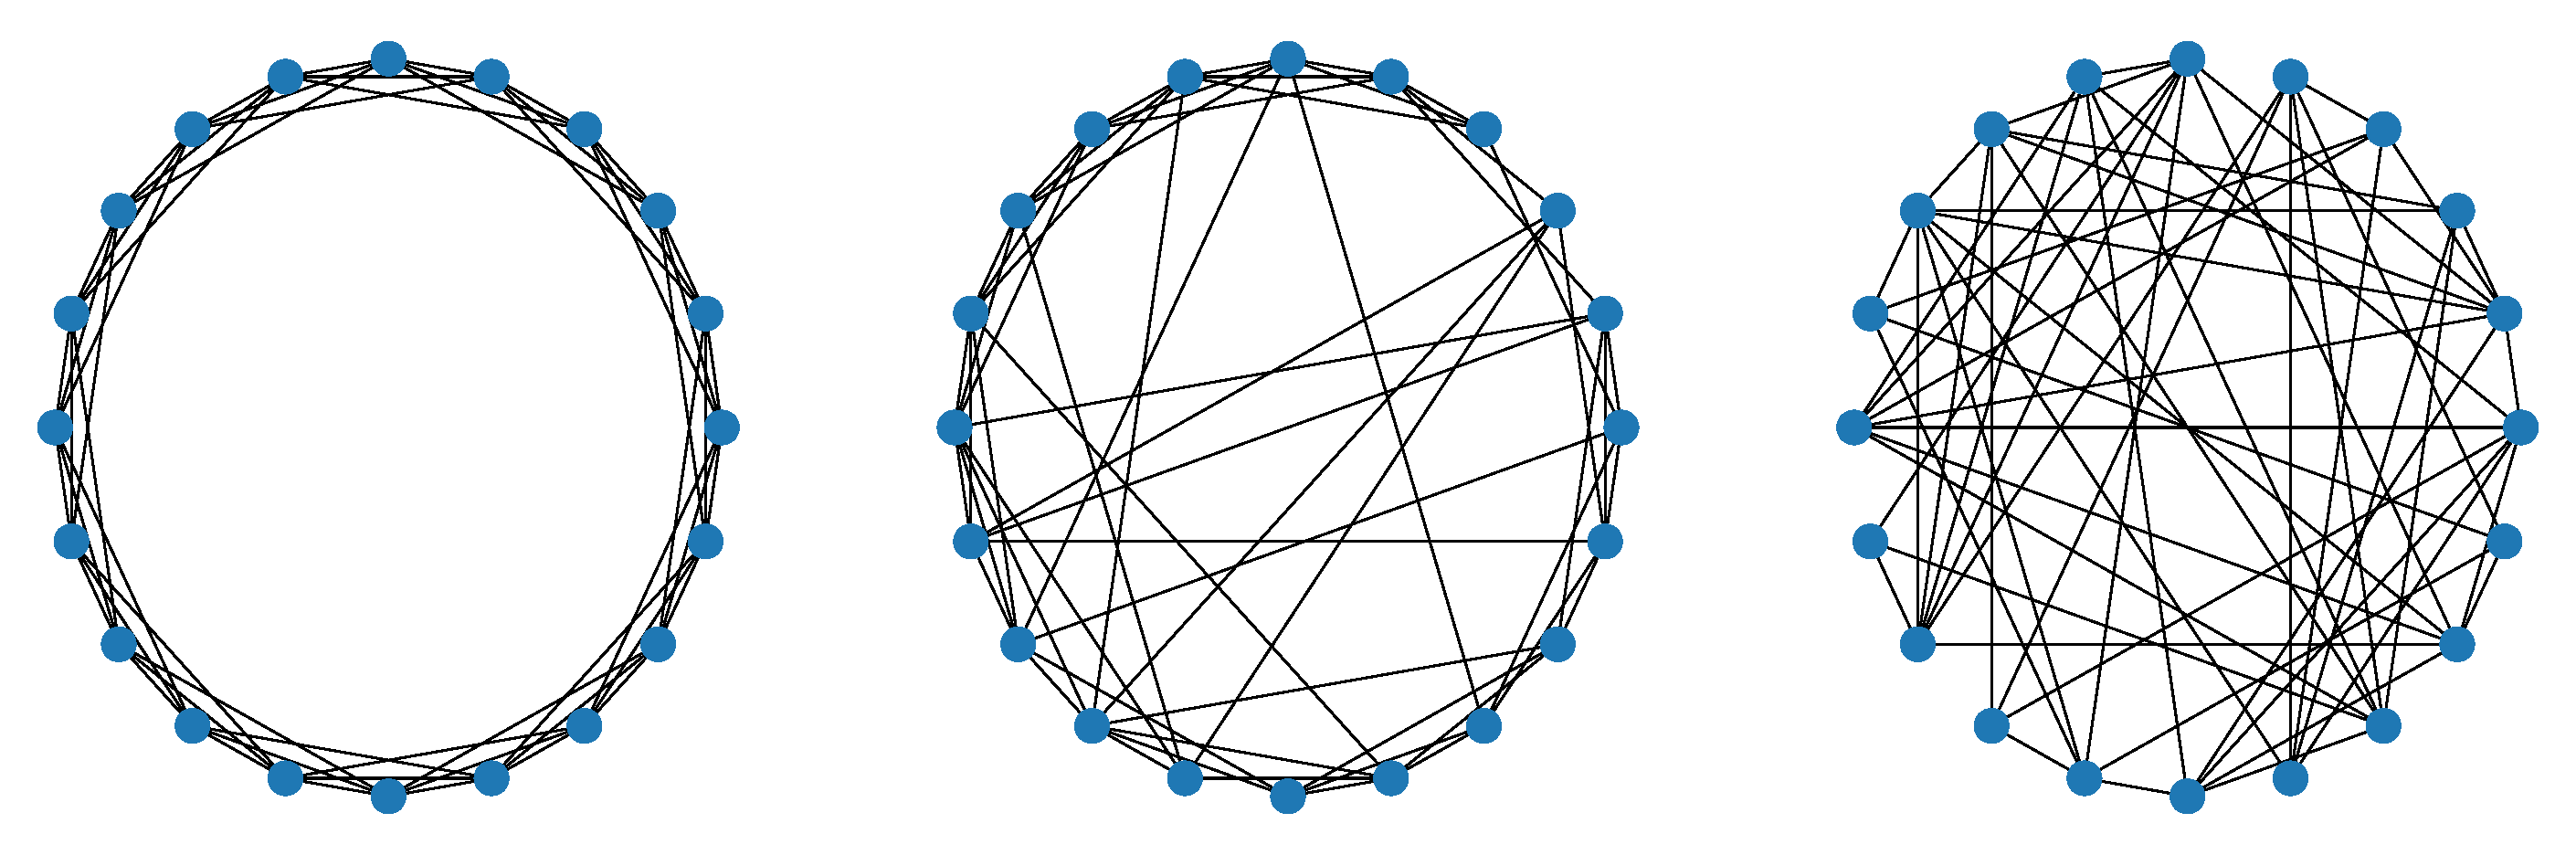
\includegraphics[width=11cm]{figs/ring_sw.pdf}
%  \end{center}
%\end{figure}
%\end{frame}

\begin{frame}\frametitle{スモールワールドネットワーク}
  \begin{itemize}
    \item スモールワールドネットワーク
    \begin{itemize}
      \item ネットワーク全体の直径が小さい
    \end{itemize}
  %\begin{itemize}
    \item \textbf{Watts--Strogatz model}\footnote{Watts and Strogatz, 1998}: スモールワールド性を記述する代表的なモデル
    \begin{itemize}
      \item \red{$O(N)$}本の枝を持つ(全結合グラフは$O(N^{2})$)
    \end{itemize}
  \end{itemize}
  \vspace{2mm}
  \hspace{2.5cm}\textbf{全結合}\hspace{3cm}\textbf{スモールワールドネットワーク}
  \vspace{0.1mm}
  \begin{figure}
    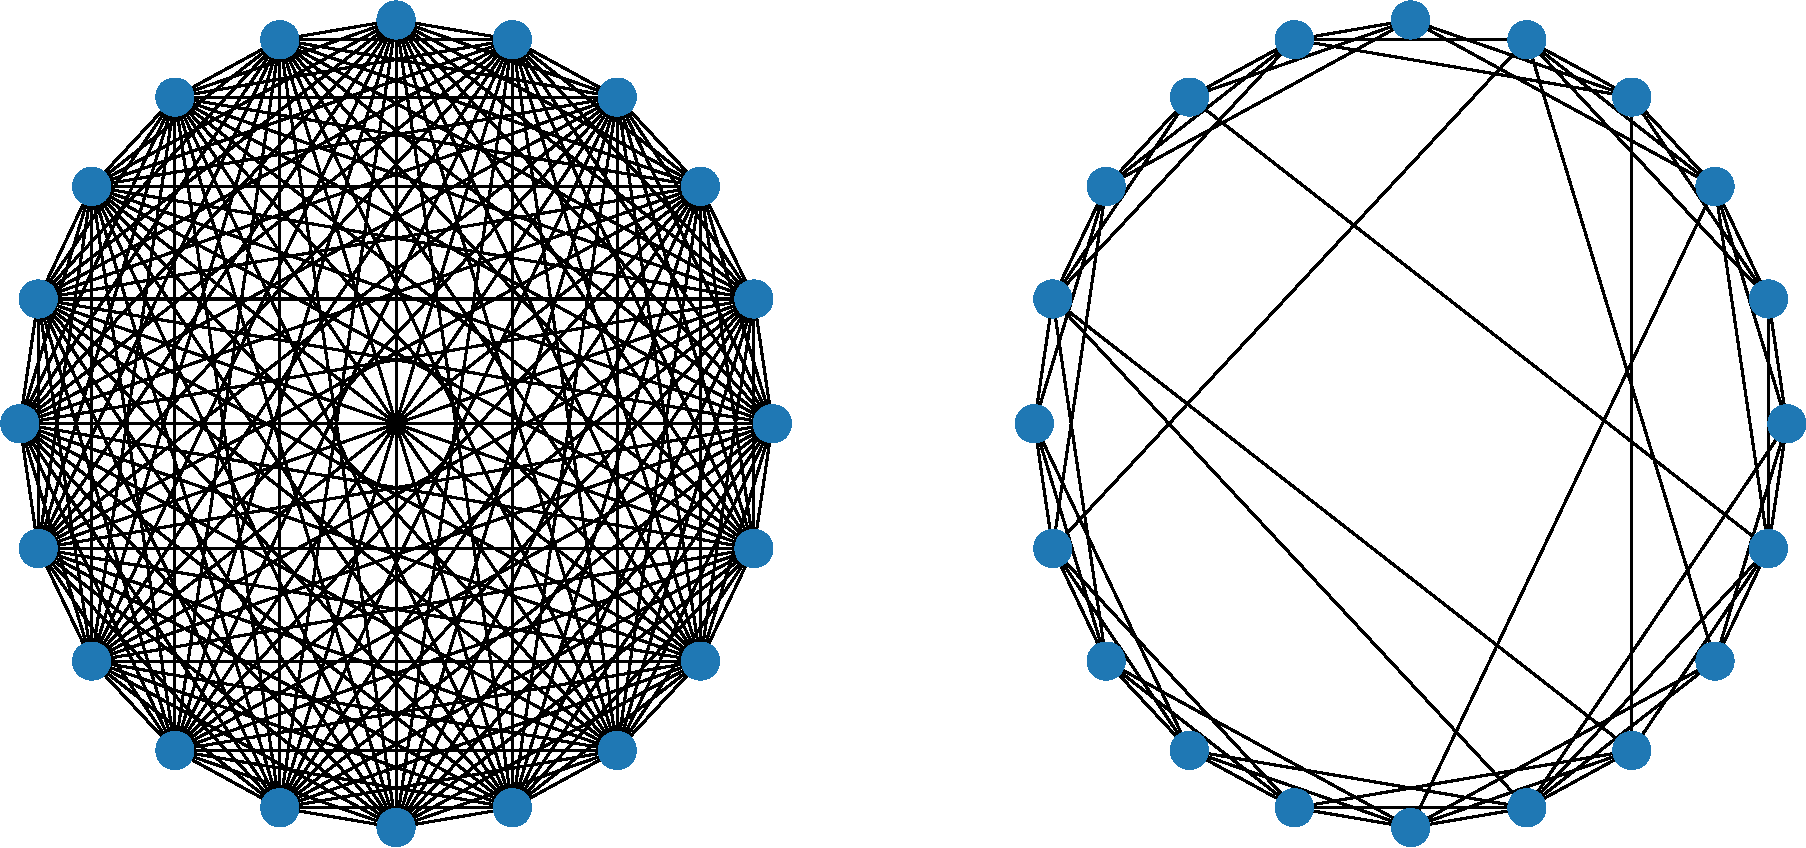
\includegraphics[width=10cm]{figs/mf_sw-crop.pdf}
  \end{figure}
\end{frame}

\begin{frame}\frametitle{スモールワールドネットワーク上の結合振動子モデル}
  \begin{block}{スモールワールドネットワーク上の結合振動子モデル}
    \begin{center}
      $\displaystyle\frac{\diff\theta_{i}}{\diff t}=\omega_{i}+\frac{K}{2k}\sum_{j\in\Lambda_{i}}\left[\sin(\theta_{j}-\theta_{i})+a\sin2(\theta_{j}-\theta_{i})\right]$
    \end{center}
    \begin{itemize}
      \item $\Lambda_{i}$: $i$番目の振動子に接続する振動子のindex集合。Watts--Strogatzモデルに従って生成したネットワークによって定まる。
      \item $k$: (ネットワークの平均次数)/$2$
    \end{itemize}
  \end{block}
  \begin{table}[htbp]
    \begin{center}
      {\tabulinesep=1.2mm
      \begin{tabu}{c||c|c|c|c|c|c}\hline\hline
       & \multicolumn{3}{c|}{all-to-all($\color{red}O(N^{2})$)} & \multicolumn{3}{c}{small-world($\color{red}O(N)$)} \\\hline
       & $a<0$ & $a=0$ & $a>0$ & $a<0$ & $a=0$ & $a>0$\\\hline\hline
      $n=1$ & $1$ & $1/2$ & (不連続) & \red{?} & \begin{tabular}{c}(\red{$1/2$})\\(Hong 2001)\end{tabular} & \red{?}\\\hline
      $n\geq 2$ & $1$ & $1/(2n)$ & (不連続) & \red{?} & \red{?} & \red{?}\\\hline
      $n=\infty$ & $1$ & (不連続) & (不連続) & \red{?} & \red{?} & \red{?}\\\hline\hline
      \end{tabu}
      }
    \end{center}
  \end{table}
\end{frame}

%\begin{frame}\frametitle{臨界指数}
%  \begin{itemize}
%    \item 結合関数が$\sin\theta$で$g(\omega)$がGaussian($n=1$)の場合に数値的に臨界指数を求めている[Hong et al. 2002]。
%  \end{itemize}
%  \begin{table}[htbp]
%    \begin{center}
%      {\tabulinesep=1.2mm
%      \begin{tabu}{c||c|c|c|c|c|c}\hline\hline
%       & \multicolumn{3}{c|}{all-to-all} & \multicolumn{3}{c}{small-world} \\\hline
%       & $a<0$ & $a=0$ & $a>0$ & $a<0$ & $a=0$ & $a>0$\\\hline\hline
%      $n=1$ & $1$ & $\dfrac{1}{2}$ & (不連続) & ? & $\red{\dfrac{1}{2}}$ & ? \\\hline
%      $n\geq 2$ & $1$ & $\dfrac{1}{2n}$ & (不連続) & ? & ? & ? \\\hline
%      $n=\infty$ & $1$ & $\left(\dfrac{2}{3}\right)$ & (不連続) & ? & ? & ? \\\hline\hline
%      \end{tabu}
%      }
%    \end{center}
%  \end{table}
%  \begin{itemize}
%    \item 全結合蔵本モデルでは$g(\omega)$や結合関数によって多様な$\beta$が得られたが、スモールワールドネットワーク上の蔵本モデルでは$\beta$がどうなる??
%    \item まずは数値的に臨界指数を求める。
%  \end{itemize}
%\end{frame}

%\begin{frame}\frametitle{千葉論文との違い}
%  [Chiba et al. 2018]の中でスモールワールドネットワーク上の蔵本モデルの計算をしているが、
%  彼らは$k=\lfloor rN\rfloor, r\in(0,0.5)$としている。
%  \begin{figure}
%    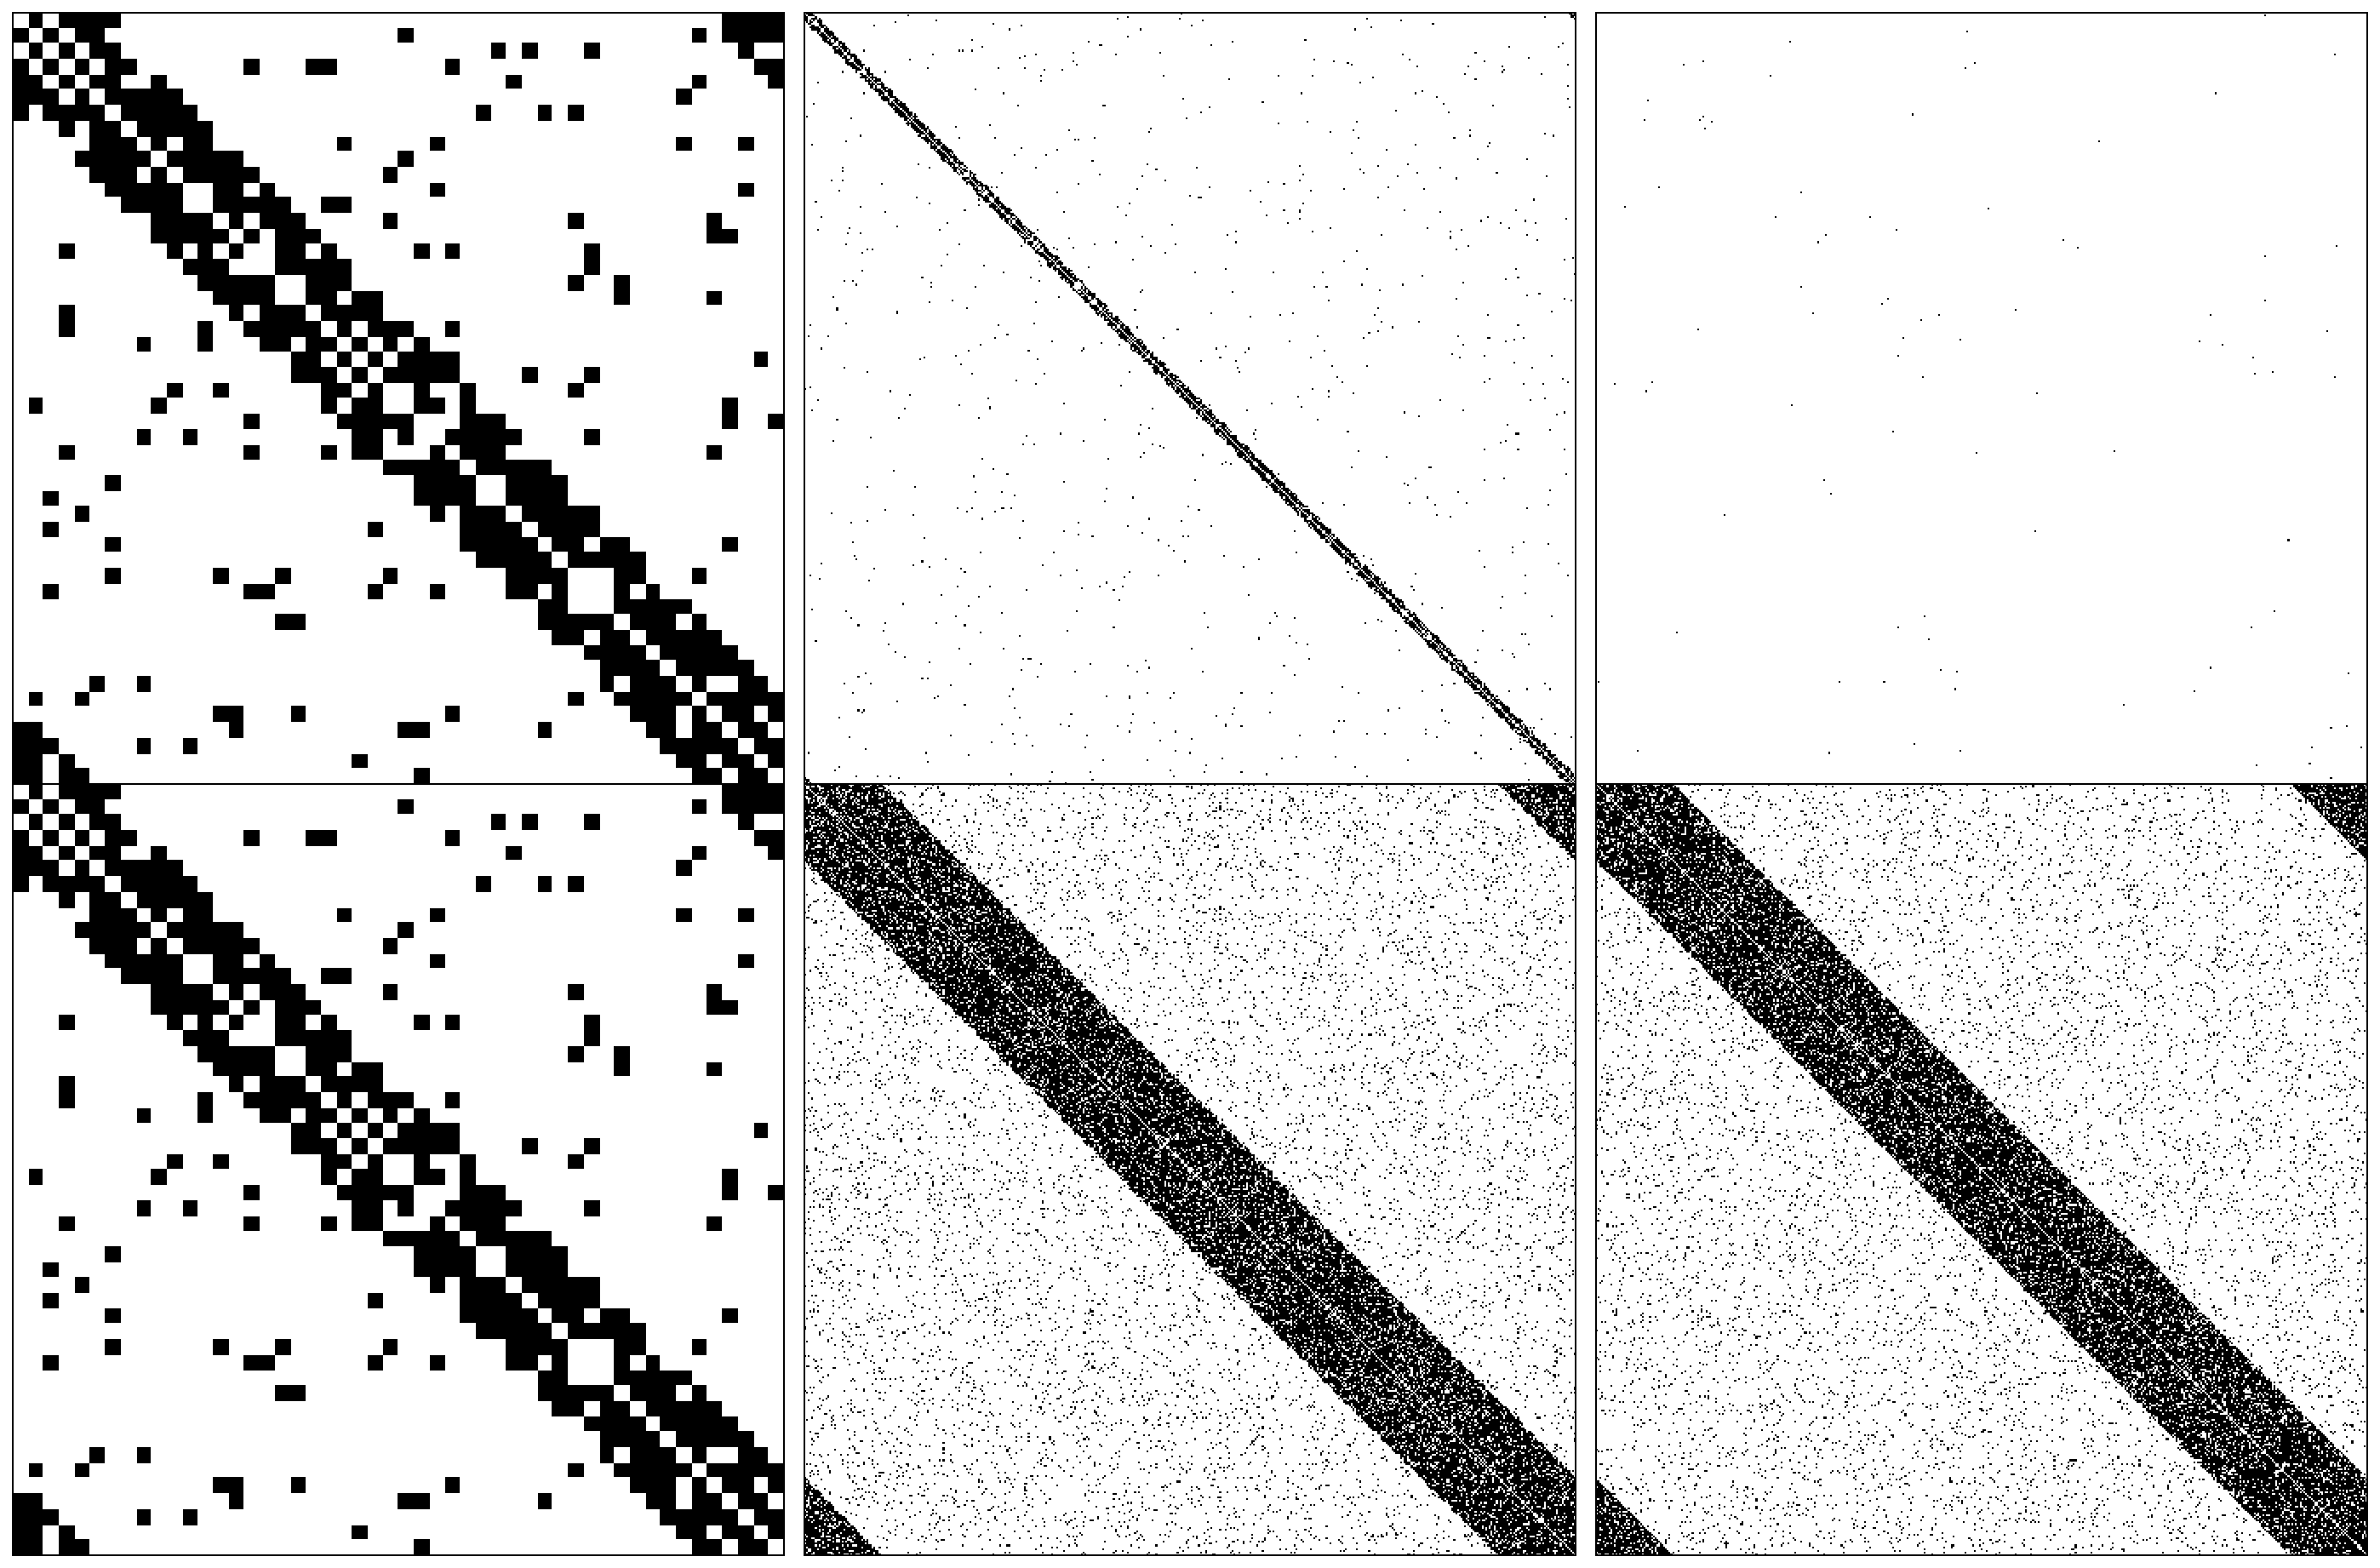
\includegraphics[scale=0.15]{figs/graphon.pdf}
%  \end{figure}
%  \begin{itemize}
%    \item $r$の立ち上がりが
%    \begin{align*}
%      r\sim\frac{C}{\sqrt{-g''(0)}}(K-\Kc)^{1/2}+\cdots
%    \end{align*}
%    \item この設定だと$\beta$が$g(\omega)$に依存することを示唆している。(全結合と変わらない結果になりうる。)
%  \end{itemize}
%\end{frame}

\begin{frame}\frametitle{有限サイズスケーリング}
  \begin{block}{有限サイズスケーリング}
    \centering
      $\displaystyle r_{N}(K)N^{\beta/\bar{\nu}}=F((K-\Kc)N^{1/\bar{\nu}})$
  \end{block}
  \begin{itemize}
    \item 連続転移する系が臨界点近傍で\textbf{スケーリング関数}$F$に従う、という仮定
    \item 有限サイズ$N$のときの$r_{N}(K)$のデータをもとに$K_{\mathrm{c}},\red{\beta},\bar{\nu}$を推定
    \begin{itemize}
      \item Bayesian scaling analysis(ガウス過程回帰を用いる)によって推定\footnote{Harada 2011}
    \end{itemize}
    \item $a=0, n=1$
    \begin{figure}
      \centering
      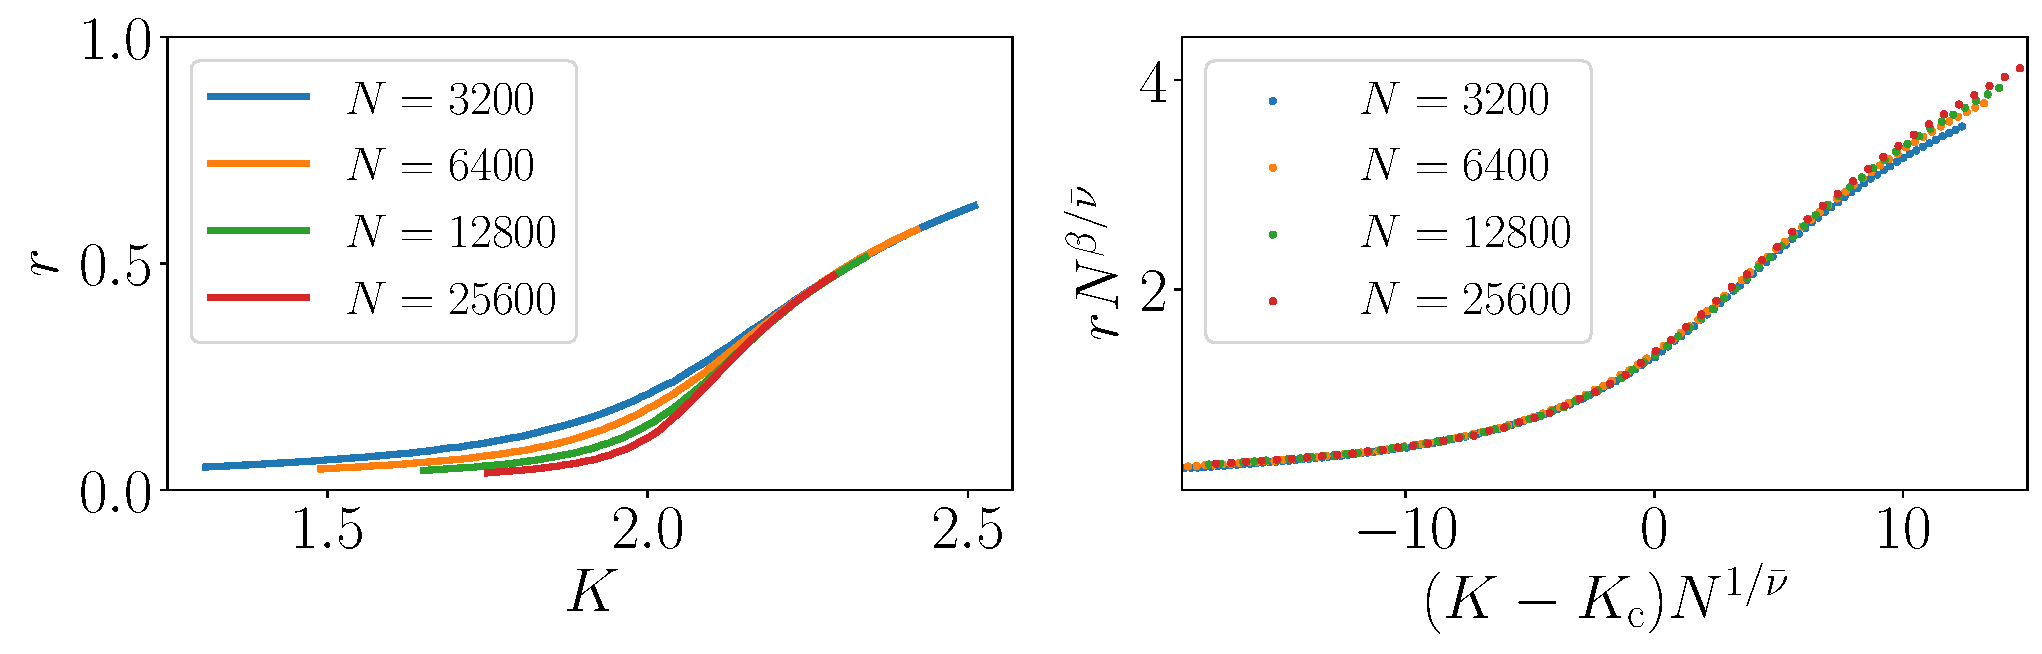
\includegraphics[width=10cm]{figs/a-0_n-1_fss.pdf}
    \end{figure}
    %\begin{align*}
    %  \frac{\beta}{\bar{\nu}}=0.215\dots,\quad
    %  \frac{1}{\bar{\nu}}=0.405\dots\quad\Rightarrow\quad
    %  \beta=0.530\dots
    %\end{align*}
  \end{itemize}
\end{frame}

%\begin{frame}\frametitle{数値計算}
%  \begin{itemize}
%    \item システムサイズを$N=100$から$N=3200$まで計算
%    \item Watts-Strogatzモデル: $(k,p)=(3,0.2)$
%    \item $\{\theta_{i}\}$の初期条件: 円周上一様ランダム
%    \item $\{\omega_{i}\}$: $g_{n}^{(G)}(\omega)$に従うようにランダムにとる($n=1,2,3,\infty$それぞれについて計算)
%    \item 時間刻み幅$\diff t=0.1$で$t=500$まで(5000ステップ)4次のRunge-Kutta法で計算
%    \item 各システムサイズに対して100回から800回計算を行う
%    \item $r$は試行回数で平均をとったものを採用
%  \end{itemize}
%\end{frame}

%\begin{frame}\frametitle{数値計算結果}
%  \begin{block}{有限サイズスケーリング}
%    \begin{align*}
%      r=N^{-\beta/\bar{\nu}}F((K-\Kc)N^{1/\bar{\nu}})
%    \end{align*}
%  \end{block}
%  \begin{itemize}
%    \item $a=0,n=1$のとき
%  \begin{figure}
%    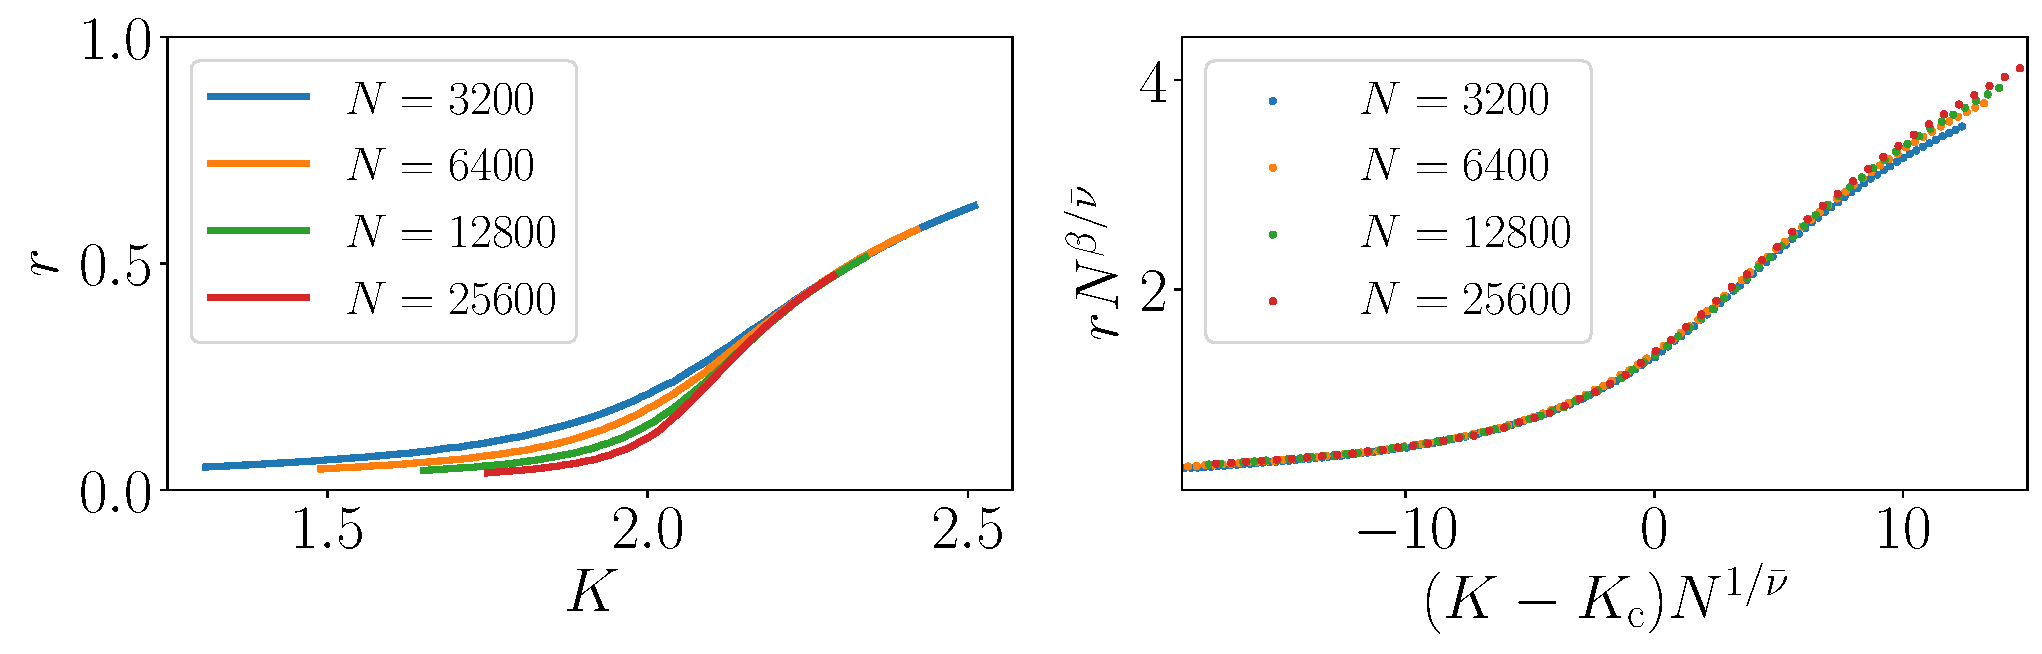
\includegraphics[width=10cm]{figs/a-0_n-1_fss.pdf}
%  \end{figure}
%  \begin{align*}
%    \frac{\beta}{\bar{\nu}}=0.2,\quad
%    \frac{1}{\bar{\nu}}=0.4\quad\Rightarrow\quad
%    \beta=0.5
%  \end{align*}
%\end{itemize}
%\end{frame}

%\begin{frame}\frametitle{数値計算結果($a=-0.2$)}
%  \begin{align*}
%    \frac{\beta}{\bar{\nu}}\approx 0.25,\quad
%    \frac{1}{\bar{\nu}}\approx 0.5\Rightarrow
%    \beta\approx \red{0.5}
%  \end{align*}
%  \begin{figure}
%    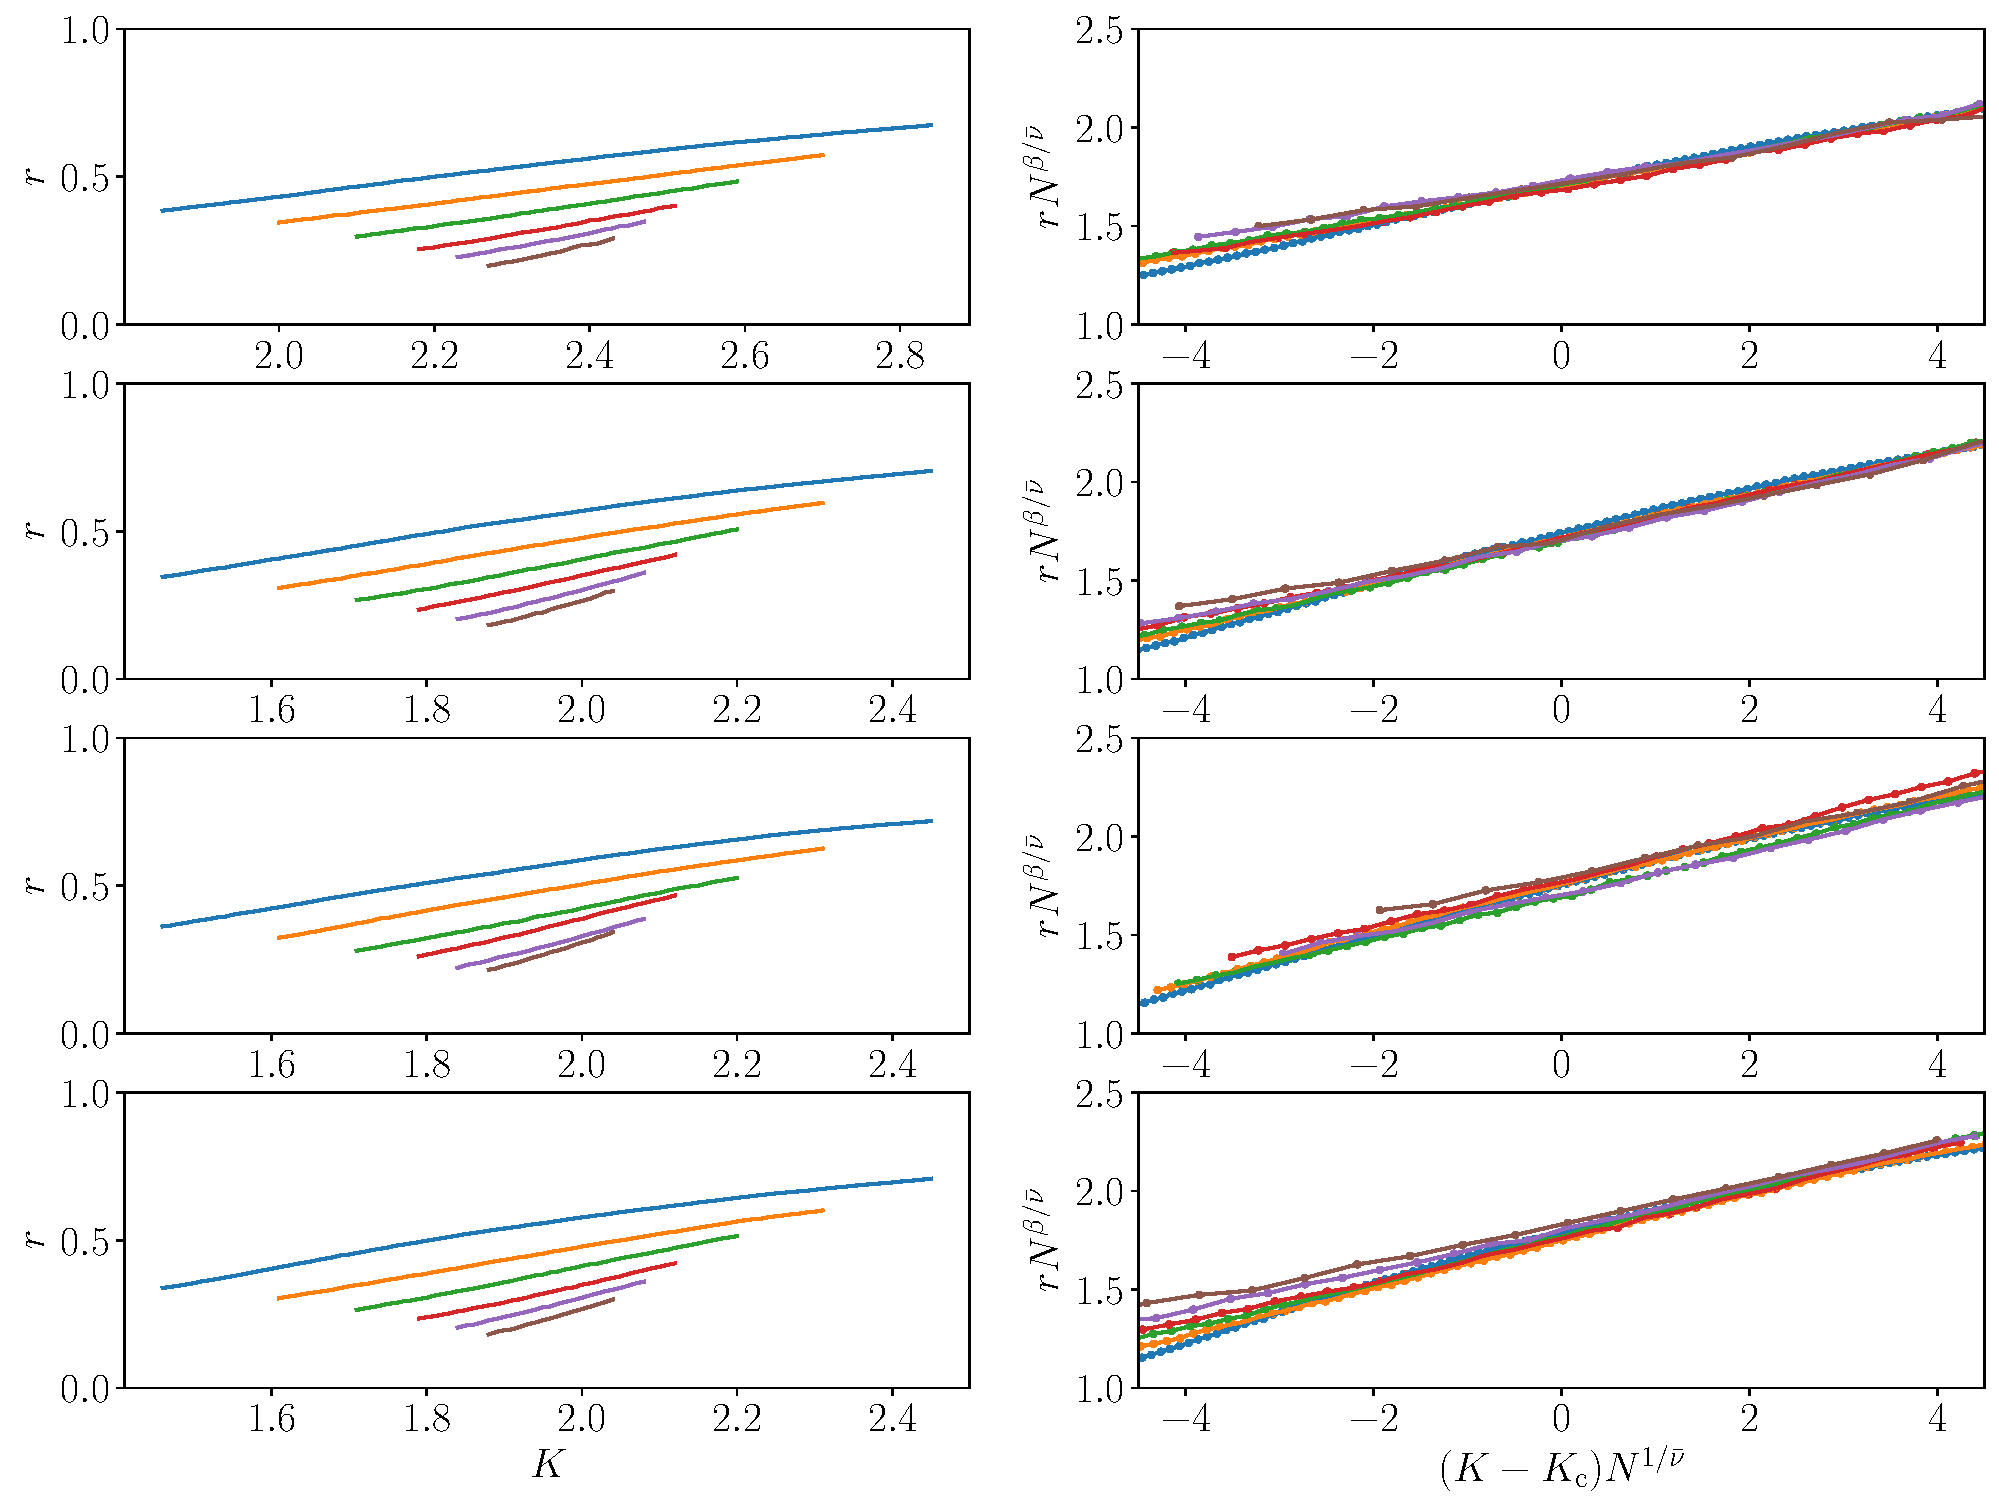
\includegraphics[width=10cm]{figs/bif-fss-sin2-a--02.pdf}
%  \end{figure}
%\end{frame}
%
%\begin{frame}\frametitle{数値計算結果($a=0.5$)}
%  \begin{align*}
%    \frac{\beta}{\bar{\nu}}\approx \red{0.15}
%  \end{align*}
%  \begin{figure}
%    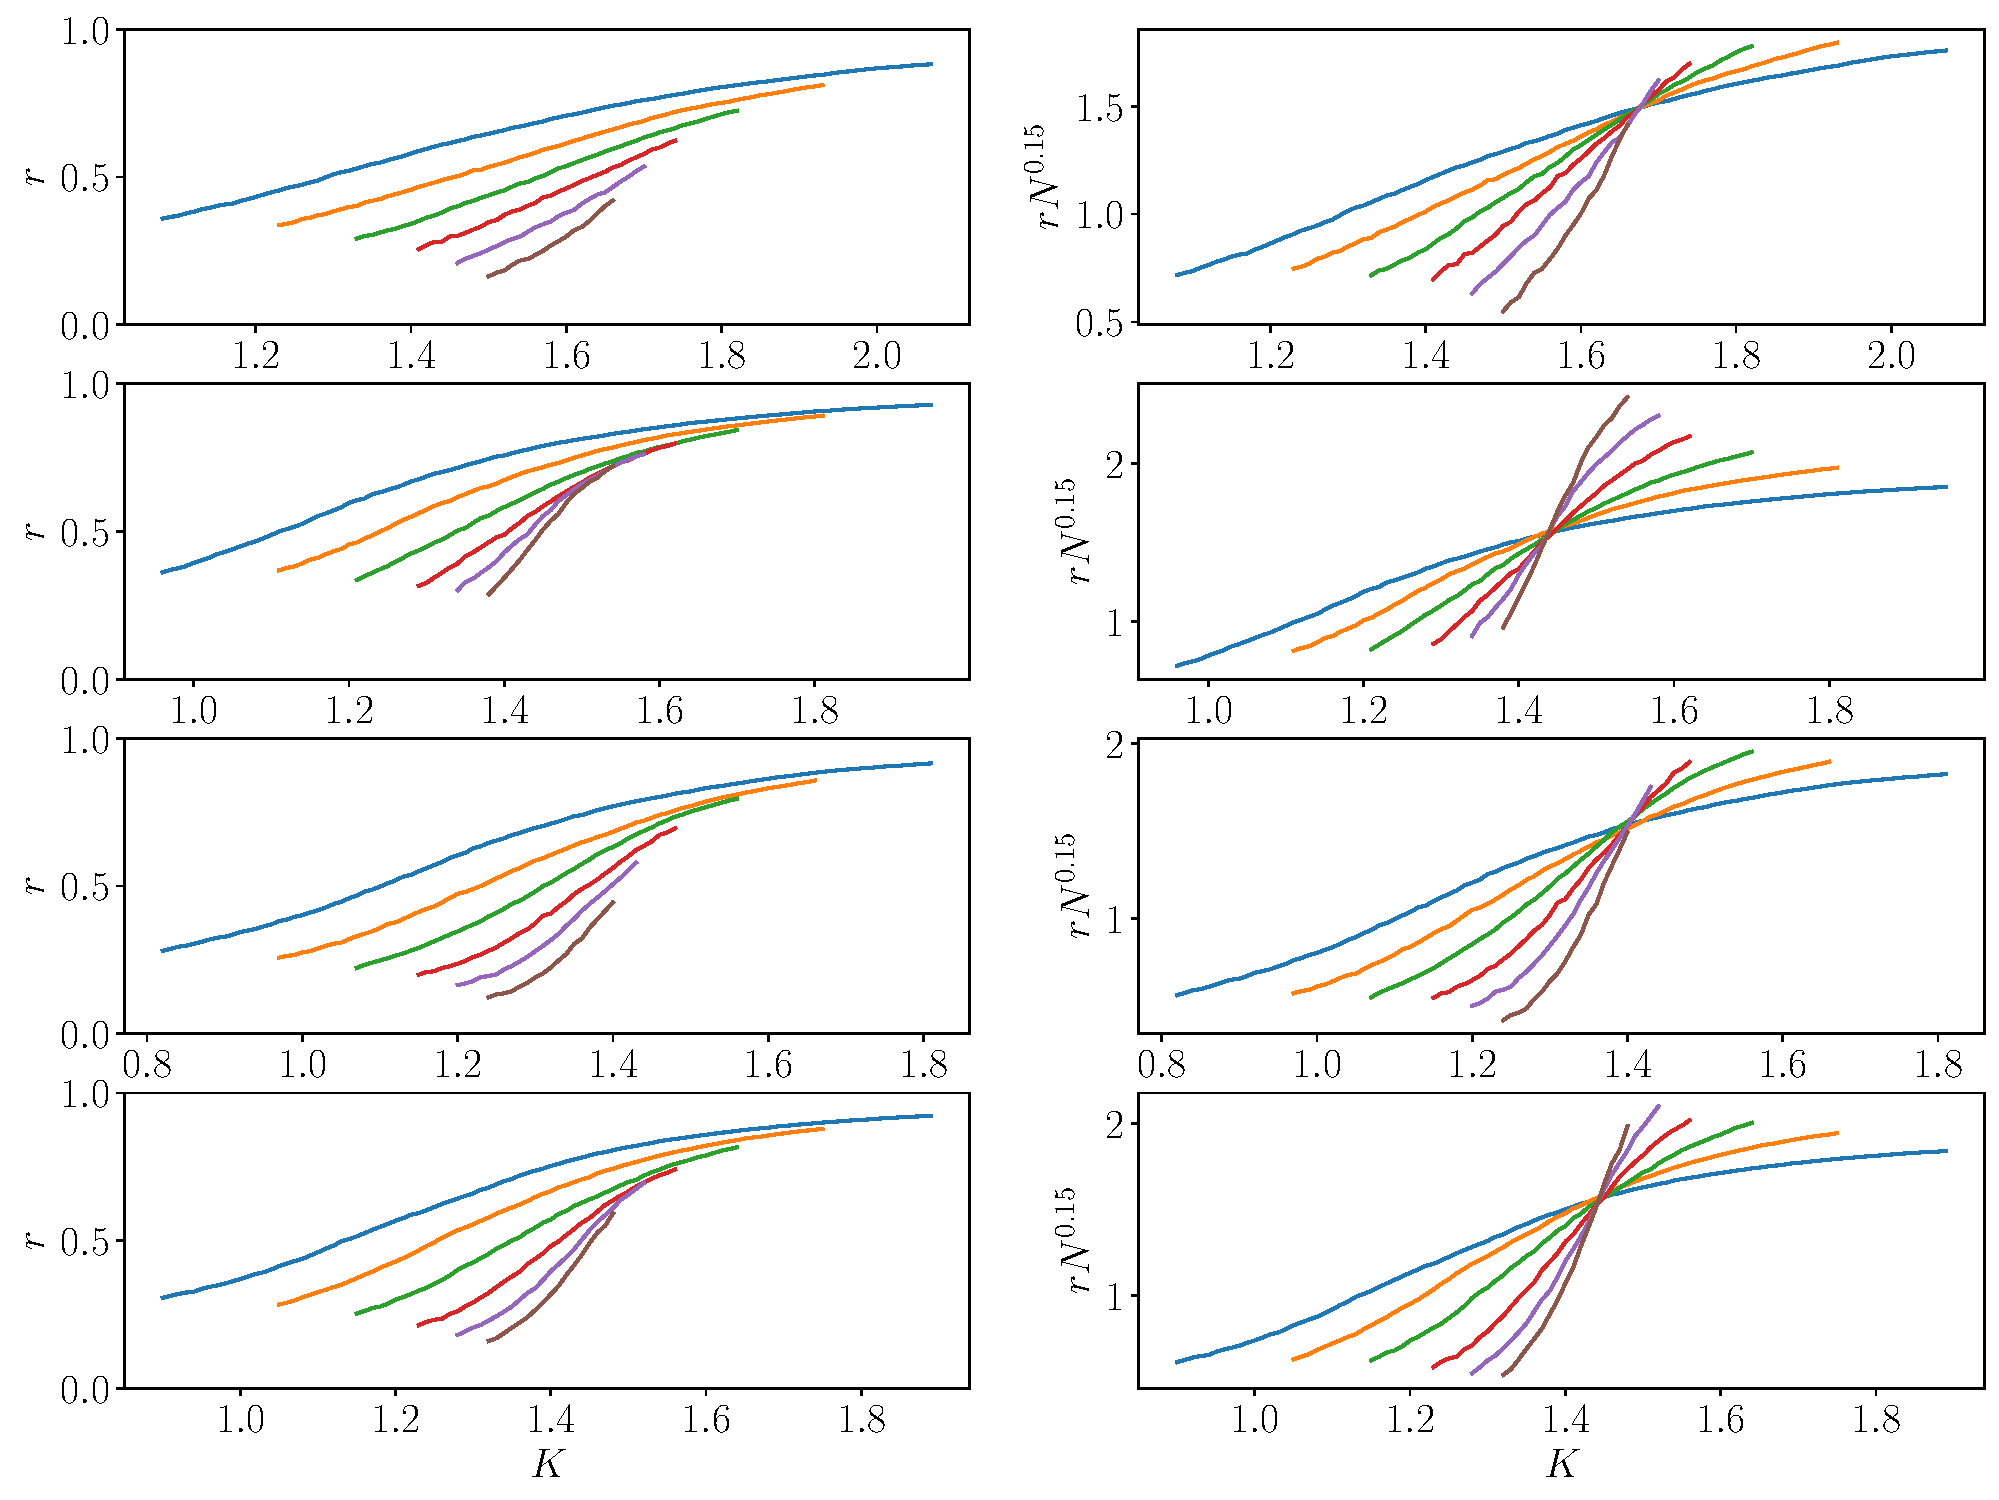
\includegraphics[width=10cm]{figs/bif-fss-sin2-a-05.pdf}
%  \end{figure}
%\end{frame}

%\begin{frame}\frametitle{微分を使った計算}
%  \begin{align*}
%    &rN^{\beta/\bar{\nu}}=const.\\
%    &\frac{\diff r}{\diff K}|_{K=\Kc}N^{(\beta-1)/\bar{\nu}}=const.
%  \end{align*}
%  \begin{figure}
%    \begin{center}
%      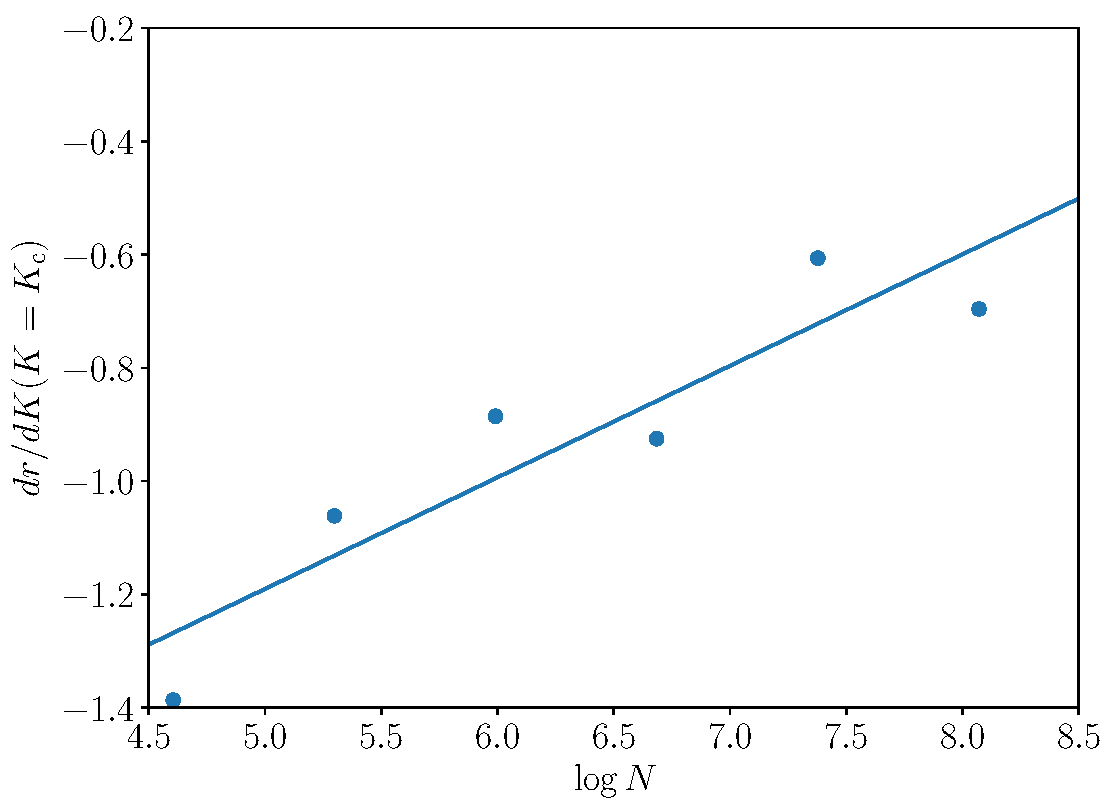
\includegraphics[width=7cm]{figs/diff-test.pdf}
%    \end{center}
%  \end{figure}
%  \begin{itemize}
%    \item 傾き$\approx 0.19$
%    \item 先行研究とのずれ
%  \end{itemize}
%\end{frame}

\begin{frame}\frametitle{数値計算結果}
  \begin{align*}
    \Gamma(\theta)=\sin\theta+{\color{blue}a}\sin2\theta,\quad
    g_{\color{red}n}(\omega)=\dfrac{ne^{-(\omega/\Delta)^{\color{red}2n}}}{\Gamma(1/2n)\Delta}
  \end{align*}
  \begin{itemize}
    \item ${\color{blue}a}=0,-0.2,0.5$と$\red{n}=1,2,3,\infty$でそれぞれ臨界指数$\beta,\bar{\nu}$を計算
    \begin{table}[thbp]
      \begin{center}
        %{\tabulinesep=1.2mm
        \begin{tabu}{cc|cccc}\hline
          $\sin\theta+\blue{a}\sin2\theta$ & $g_{{\color{red}n}}(\omega)$ & $\beta$ & & $\bar{\nu}$ &\\\hline\hline
          \multirow{4}{*}{${\color{blue}a}=0$} & $\red{n}=1$ & $0.51(4)$ & \multirow{4}{*}{$\approx\red{\dfrac{1}{2}}$} & $2.40(6)$ & \multirow{4}{*}{$\approx\red{\dfrac{5}{2}}$}\\
           & $\red{n}=2$ & $0.49(2)$ & & $2.43(4)$ &\\
           & $\red{n}=3$ & $0.47(2)$ & & $2.46(4)$ &\\
           & $\red{n}=\infty$ & $0.46(2)$ & & $2.46(4)$ &\\\hline
           \multirow{4}{*}{${\color{blue}a}=-0.2$} & $\red{n}=1$ & $0.48(6)$ & \multirow{4}{*}{$\approx\red{\dfrac{1}{2}}$} & $2.36(8)$ & \multirow{4}{*}{$\approx\red{\dfrac{5}{2}}$}\\
           & $\red{n}=2$ & $0.51(4)$ & & $2.41(6)$ & \\
           & $\red{n}=3$ & $0.55(4)$ & & $2.50(6)$ &\\
           & $\red{n}=\infty$ & $0.49(4)$ & & $2.49(6)$ &\\\hline
        \end{tabu}
        %}
      \end{center}
    \end{table}
    % \item $n$によらず
    % \begin{align*}
    %   \beta\approx\frac{1}{2},\quad\bar{\nu}\approx\frac{5}{2}
    % \end{align*}
    % \item $a=0.5$では?
    \item $a=0.5$ではヒステリシスを確認$\Longrightarrow$\textbf{不連続転移}を示唆
  \end{itemize}
\end{frame}

\begin{frame}\frametitle{まとめと展望}
  \begin{align*}
    \Gamma(\theta)=\sin\theta+{\color{blue}a}\sin2\theta,\quad
    g_{\color{red}n}(\omega)=\dfrac{n}{\Gamma(1/2n)\Delta}e^{-(\omega/\Delta)^{\color{red}2n}}
  \end{align*}
  \begin{table}[htbp]
    \begin{center}
      {\tabulinesep=1.2mm
      \begin{tabu}{c||c|c|c|c|c|c}\hline\hline
        & \multicolumn{3}{c|}{all-to-all($\color{red}O(N^{2})$)} & \multicolumn{3}{c}{small-world($\color{red}O(N)$)} \\\hline
       & $a<0$ & $a=0$ & $0<a<1$ & $a=-0.2$ & $a=0$ & $a=0.5$\\\hline\hline
      $n=1$ & $1$ & $\dfrac{1}{2}$ & (不連続) & \red{$\dfrac{1}{2}$} & \red{$\dfrac{1}{2}$} & \red{(不連続)}\\\hline
      $n\geq 2$ & $1$ & $\dfrac{1}{2n}$ & (不連続) & \red{$\dfrac{1}{2}$} & \red{$\dfrac{1}{2}$} & \red{(不連続)}\\\hline
      $n=\infty$ & $1$ & (不連続) & (不連続) & \red{$\dfrac{1}{2}$} & \red{$\dfrac{1}{2}$} & \red{(不連続)}\\\hline\hline
      \end{tabu}
      }
    \end{center}
  \end{table}
  \begin{itemize}
    \item 全結合とスモールワールドネットワークで$\beta$が異なることがわかった。
    \begin{itemize}
      \item ノイズ系と同じ臨界指数
    \end{itemize}
    \item 理論的に臨界指数を求めたい。
    \begin{itemize}
      \item 連続極限をどう取る??(graphonを用いた解析はできない)
    \end{itemize}
  \end{itemize}
\end{frame}